% !TeX program = pdfLaTeX
\documentclass[12pt]{article}
\usepackage{amsmath}
\usepackage{graphicx,psfrag,epsf}
\usepackage{enumerate}
\usepackage{natbib}
\usepackage{textcomp}
\usepackage[hyphens]{url} % not crucial - just used below for the URL
\usepackage{hyperref}
\providecommand{\tightlist}{%
  \setlength{\itemsep}{0pt}\setlength{\parskip}{0pt}}

%\pdfminorversion=4
% NOTE: To produce blinded version, replace "0" with "1" below.
\newcommand{\blind}{0}

% DON'T change margins - should be 1 inch all around.
\addtolength{\oddsidemargin}{-.5in}%
\addtolength{\evensidemargin}{-.5in}%
\addtolength{\textwidth}{1in}%
\addtolength{\textheight}{1.3in}%
\addtolength{\topmargin}{-.8in}%

%% load any required packages here




\usepackage{longtable}
\usepackage[utf8]{inputenc}
\usepackage{polski}
\usepackage[polish]{babel}
\usepackage[nosingleletter]{impnattypo}
\usepackage{amsmath}
\usepackage{mathtools}
\usepackage{parskip}
\setlength{\parskip}{\baselineskip}
\setlength{\parindent}{0pt}
\usepackage{caption}
\captionsetup[table]{name=Tabela}
\usepackage{booktabs}
\usepackage{longtable}
\usepackage{array}
\usepackage{multirow}
\usepackage{wrapfig}
\usepackage{float}
\usepackage{colortbl}
\usepackage{pdflscape}
\usepackage{tabu}
\usepackage{threeparttable}
\usepackage{threeparttablex}
\usepackage[normalem]{ulem}
\usepackage{makecell}
\usepackage{xcolor}

\addto\captionspolish{
  \renewcommand{\listtablename}
    {Spis tabel}
}

\begin{document}


\def\spacingset#1{\renewcommand{\baselinestretch}%
{#1}\small\normalsize} \spacingset{1}


%%%%%%%%%%%%%%%%%%%%%%%%%%%%%%%%%%%%%%%%%%%%%%%%%%%%%%%%%%%%%%%%%%%%%%%%%%%%%%

\if0\blind
{
  \begin{center}
  
\includegraphics{AGHlogo.jpg}\\[2ex]
    \textbf{\normalsize WYDZIAŁ ZARZĄDZANIA}

  \normalsize{PRACOWNIA ZASTOSOWAŃ MATEMATYKI W EKONOMII}
  \end{center}
\vspace{1cm}
  \begin{center}
    \large{Praca dyplomowa  magisterska}
  \end{center}
\vspace{1cm}
\begin{center}
  \large{\bf Zagadnienie równoważności pomiarowej w badaniach różnic w postrzeganiu demokracji w UE.}

  \large{\bf The problem of measurement invariance in the reaserch of differences in attitude toward democracy in the EU.
}
\end{center}
\bigskip
\vspace{2cm}
\begin{tabbing}
\hspace{5cm} \= \hspace{5cm} \\
Autor:	 \> Agnieszka Choczyńska \\
Kierunek studiów: \>  Informatyka i Ekonometria \\
Opiekun pracy: \> dr Jacek Wolak \\
\end{tabbing}

\begin{center}
	Kraków, 2020
\end{center}

} \fi

\if1\blind
{
  \bigskip
  \bigskip
  \bigskip
  \begin{center}
    {\LARGE\bf Zagadnienie równoważności pomiarowej w badaniach różnic w postrzeganiu demokracji w UE.}
  \end{center}
  \medskip
} \fi


\newpage
\spacingset{1.45} % DON'T change the spacing!

\tableofcontents
\listoftables
\listoffigures

\newpage

\hypertarget{wprowadzenie}{%
\section*{Wprowadzenie}\label{wprowadzenie}}
\addcontentsline{toc}{section}{Wprowadzenie}

Słowo ``demokracja'' jest odmieniane przez wszystkie przypadki w deklaracjach polityków, na demonstracjach, w mediach i w codziennych rozmowach. Niejednokrotnie przedmiot tych wypowiedzi wychodzi daleko poza zwięzłą, przyjętą przez politologów definicję, tj. demokracja to system, w którym obywatele mogą przyjąć lub odrzucić elity mające nimi rządzić \citep{Schumpeter}. Rozdźwięk między formalną definicją a społecznym postrzeganiem zjawiska nie jest niczym niezwykłym, jednak w tym przypadku nabiera szczególnego znaczenia. Choć Ziemia nie przestanie krążyć wokół Słońca, nawet gdyby cała ludzkość uważała inaczej, to kształt systemów demokratycznych zależy od tego, jak ich obywatele wyobrażają sobie demokrację.

Problem ma szczególne znaczenie w badaniach naukowych, w których dokonywana jest ocena demokratyczności państw lub nastawienia do demokracji grup czy całych społeczeństw, aby następnie porównywać je między sobą. Jest to zawsze odniesienie do jednej, eksperckiej koncepcji demokracji, więc nie pozwala na pełne zrozumienie wyborów ludzi, którzy kierują się funkcjonującymi w ich społecznościach koncepcjami, niekoniecznie ``poprawnymi'' i niekoniecznie ponadnarodowymi.

Dlatego jest tak ważne, żeby wciąż badać, czym demokracja w społecznym przekonaniu tak naprawdę jest. Ta praca stawia sobie na cel eksplorację przekonań mieszkańców Europy na temat istoty demokracji, wyrażonych w odpowiedziach na ankietę World Values Survey. Na tej podstawie zostanie podjęta próba skonstruowania społecznych koncepcji demokracji, pozwalających wyrazić liczbowo siłę tych przekonań.

Struktura pracy jest następująca: w pierwszym rozdziale przedstawiono pokrótce dotychczasowe sposoby definiowania i mierzenia demokracji, zarówno na podstawie wiedzy eksperckiej jak i dzięki analizie danych zebranych w badaniach społecznych. W rozdziale drugim omówiono model analizy czynnikowej, który zostanie wykorzystany w badaniu, oraz zagadnienie równoważności pomiarowej, która jest warunkiem przeprowadzania analizy międzygrupowej. W następnych rozdziałach opisano kolejne etapy badania wraz z wynikami i wnioskami z analizy.

\newpage

\hypertarget{iloux15bciowe-badania-nad-demokracjux105-w-literaturze-przedmiotu}{%
\section{Ilościowe badania nad demokracją w literaturze przedmiotu}\label{iloux15bciowe-badania-nad-demokracjux105-w-literaturze-przedmiotu}}

\hypertarget{motywacje-iloux15bciowego-badania-demokracji}{%
\subsection{Motywacje ilościowego badania demokracji}\label{motywacje-iloux15bciowego-badania-demokracji}}

W tym rozdziale zostaną omówione powszechnie przyjmowane definicje demokracji, sposoby mierzenia jakości demokracji i wyrażania jej za pomocą liczbowych wskaźników. Poruszona zostanie także kwestia problemów ograniczeń, jakie wiążą się ze stosowaniem takiego podejścia.

Potrzeba ilościowego wyrażenia stopnia zdemokratyzowania państwa narodziła się w drugiej połowie XX wieku w Stanach Zjednoczonych Ameryki. Według panującego wówczas paradygmatu, państwa demokratyczne charakteryzują się mniejszą skłonnością do prowadzenia wojen, zwłaszcza przeciwko innym demokracjom. Dla ludzi odpowiedzialnych za politykę zagraniczną USA, podwyższenie poziomu demokracji w kluczowych regionach było niezbędne do zapewnienia pokoju \citep{Doorenspleet}.

Stąd zrodziła się potrzeba stworzenia wskaźnika demokratyczności, który pozwalałby porównywać państwa pod tym kątem, określać, jak daleko są od ``idealnej'' demokracji, oraz oceniać po czasie wyniki podjętych działań. Wyrażenie takiej własności liczbą otwiera również szerokie możliwości tworzenia modeli, w których stopień zdemokratyzowania państwa występuje jako zmienna objaśniana lub objaśniająca, co pozwala wyjaśniać przyczyny, skutki i własności demokracji w sposób dużo bardziej ścisły, poprawny metodologicznie oraz możliwy do zreprodukowania przez innych badaczy.

Między innymi dzięki tym możliwościom, bezpośredni związek stopnia demokratyzacji państwa z jego skłonnością do wojen został przez wielu badaczy podważony lub uznany za słabszy niż inne czynniki, np. wolnorynkowość czy stabilność struktur władzy \citep{Doorenspleet}. Wciąż, demokracja jest przedmiotem intensywnych badań socjologów i politologów. A fakt, że badacze interesują się zrozumieniem zjawiska samego w sobie, a nie tylko kontekstem polityki zagranicznej danego państwa, wymusza bliższe przyjrzenie się kwestii obiektywności takich badań.

Zachowanie obiektywności nie jest w tym przypadku proste, z kilku powodów.

Po pierwsze, ustrój polityczny dotyczy tak wielkich jednostek jak państwa, wobec czego badania nad demokracją, które muszą uwzględnić wiele krajów, borykają się ze wszystkimi problemami dotyczącymi różnic kulturowych i językowych.

Po drugie, problematyczna jest sama kwestia definiowania demokracji. W klasycznym rozumieniu jej istotą była władza w rękach ludu, nadanie obywatelom prawa do decydowania o sprawach politycznych. W latach 40. XX w. zaczęło dominować alternatywne podejście, zaproponowane przez J. Schumpetera. Jego zdaniem, \emph{``demokracja oznacza tylko tyle, że ludzie mają możliwość zaakceptować lub odrzucić tych, którzy mają nimi rządzić''} \citep{Schumpeter}. Społeczeństwo jako całość nie musi w jakikolwiek czynny sposób angażować się w politykę; jedynie wyznaczać elity, które będą się tym zajmować. Partycypacja, kluczowa w klasycznej definicji, dla Schumpetera była nieistotna, lub nawet szkodliwa. Taką koncepcję nazywa się elektoralną.

Wymienia się jeszcze kilka innych, szeroko wykorzystywanych podejść, które przedstawia Tabela 1.

\begin{table}

\begin{longtable}[t]{l|>{\raggedright\arraybackslash}p{30em}}
\caption{\label{tab:dem-types}Koncepcje demokracji. Źródło: Coppedge et al. 2011}\\
\hline
Typ demokracji &  Postulaty\\
\hline
liberalna & wolności obywatelskie, prawa mniejszości, praworządność i przejrzystość, możliwość kontrolowania rządzących\\
\hline
większościowa & najważniejsza jest wola większości, silna, jednostkowa władza\\
\hline
bezpośrednia & jak największy udział obywateli w bezpośrednim podejmowaniu decyzji (w kontraście do wybierania przedstawicieli)\\
\hline
deliberatywna & decyzje podejmowane w drodze dyskusji i wypracowywania konsensusu (w kontraście do przegłosowania przeciwników)\\
\hline
egalitarna & równość w prawach, ale też dostępie do zasobów; każdy obywatel ma szansę w takim samym stopniu korzystać ze wspólnego państwa\\
\hline
\end{longtable}
\end{table}

Po trzecie wreszcie, badacze zauważają, że pojęcie demokracji jest silnie nacechowane emocjonalnie \citep{JaskoKoss}. Ludzie mają skłonność do uznawania demokracji nie za jedną z możliwych form systemu politycznego, ale raczej za stan idealny. Stąd tak wiele państw, które mają demokrację w nazwie, a są powszechnie uważane za autorytarne. Można by powiedzieć w uproszczeniu, że ludzie zawsze są za demokracją, tylko zazwyczaj ta demokracja ma niewiele wspólnego z którąkolwiek z definicji. Z jednej strony powoduje to przypisanie do czysto politycznego pojęcia demokracji licznych postulatów o charakterze gospodarczym czy etycznym. Z drugiej, przyjęcie jednej definicji, stworzonej przez człowieka ukształtowanego w określonej kulturze, zamyka na faktyczną różnorodność zjawiska demokracji.

Według minimalistycznej definicji, istotą demokracji jest mechanizm wykorzystania argumentu siły bez używania przemocy. Akceptuje się wolę większości, nie dlatego, że większość ma rację, ale dlatego, że bunt wobec tej woli oznacza bunt wobec przeważającej siły - mimo, że współcześnie siła zależy bardziej od przewagi technicznej niż liczebności \citep{Przeworski}. Głos jest walutą władzy; demokracja była rewolucją ustrojową na miarę wynalezienia pieniądza w gospodarce. Jak jednak zauważa dalej Przeworski, trwałość i jakość demokracji zależą od szeregu czynników, zarówno politycznych, jak i ekonomicznych. Dlatego warto spróbować określić istotę demokracji nie od strony mechanizmu przekazywania władzy, ale od strony oczekiwań, jakie ma ten mechanizm spełnić. Ponieważ właśnie to, a nie minimalistyczna definicja, może pomóc odpowiedzieć na pytanie, dlaczego demokracja bywa popierana albo odrzucana.

\hypertarget{wskaux17aniki-demokracji}{%
\subsection{Wskaźniki demokracji}\label{wskaux17aniki-demokracji}}

Zdecydowana większość wskaźników demokracji jest tworzona na podstawie oceny ekspertów. Obliczenie wartości polega na przyznaniu państwu punktów za każdy spełniony standard demokratyczny oraz pewną procedurę agregacji. To oznacza, że każdy przypadek porównuje się z pewną, wybraną przez twórców metody, koncepcją demokracji. Istnieją wskaźniki oceniające państwa według minimalistycznej koncepcji, w skali binarnej (jest demokracją lub nie jest), ale ze względu na swoją prostotę mają zastosowanie głównie przy badaniu ciągłości demokracji \citep{Coppedge}. Do celu porównywania ze sobą różnych państw demokratycznych powstały inne wskaźniki, oparte o węższe koncepcje.

Jeden z najczęściej używanych jest obliczany co roku przez amerykańską organizację Freedom House, powiązaną z CIA \citep{Doorenspleet}. Freedom House Index (FH) wykorzystuje 7-stopniową skalę do oceny praw politycznych oraz obywatelskich (im niższa ocena, tym lepiej). Pomimo, że według intencji twórców nie miał być nawet wskaźnikiem demokracji, to jest jako taki powszechnie wykorzystywany przez badaczy \citep{Coppedge}, ponieważ wyraża własności obecnie dominującej koncepcji liberalnej. Inne wskaźniki mogą nieco różnić się konstrukcją oraz skalą, ale generalnie opierają się o tę samą metodykę.

Przede wszystkim zakładają, że przeciwieństwem demokracji jest system autorytarny, i pozwalają umiejscowić każde badane państwo na osi autorytaryzm - demokracja. Przejście jest tonalne, nie ma ścisłego punktu, od którego kraj jest klasyfikowany jako któraś z tych dwóch opcji. Ponadto mniej więcej środek skali określa się jako odrębny typ ustroju, tak zwaną demokrację hybrydową, w której łączą się pewne rozwiązania z obu skrajnych typów \citep{Doorenspleet}.

Wskaźniki demokracji weszły do powszechnego użytku, ale doczekały się też krytyki. Argumentowano, że zbyt mocno opierają się na procedurach i formalnym stanie prawnym, a za mało na stanie faktycznym, oraz że zbyt ogólne i niejednoznaczne kryteria pozwalają wystawiającym ocenę projektować swoje wyobrażenia o demokratyczności państw na liczbę punktów \citep{Coppedge}. Szczególnie wobec FH pojawiły się również zarzuty konserwatywnego i pro-rynkowego skrzywienia, oraz zaniżania oceny dla lewicowych i muzułmańskich rządów \citep{Doorenspleet}. To by oznaczało, że wskaźnik nie ocenia wyłącznie stopnia spełnienia bardzo szerokiej, lecz precyzyjnej definicji, ale też nie uwzględnia całej istniejącej różnorodności systemów demokratycznych.

\hypertarget{spoux142eczna-koncepcja-demokracji}{%
\subsection{Społeczna koncepcja demokracji}\label{spoux142eczna-koncepcja-demokracji}}

Zupełnie innym podejściem do mierzenia demokracji jest oparcie wskaźnika o zdanie samych obywateli. Nie jest to alternatywny sposób na osiągnięcie tego samego celu, ale raczej próba badania demokracji takiej, jaka jest - niekoniecznie zgodnej z definicją, za to odzwierciedlającej zamysł ludzi, którzy ją wprowadzali i podtrzymywali.

Jak wskazuje \citet{Campbell}, u podstaw poparcia dla demokracji i demokratycznych rządów leży proces modernizacji, który dotknął każdej dziedziny ludzkiego życia, przez co zmiany stały się właściwie ``sprawą każdego''. Jako wskazywane przez badaczy wyjaśnienia tego poparcia podaje: a)\(~\)zaangażowanie w działalność społeczną, która \emph{``zapewnia antidotum na uczucie apatii i alienacji, oraz projektuje atmosferę zaufania na organy rządowe''}\footnote{Tłumaczenie własne}, b)\(~\)czynniki ekonomiczne - sprzyjająca sytuacja powoduje wyższe poparcie, które spada w trudniejszych czasach, c)\(~\)czynniki behawioralne, które powodują, że ludzie generalnie popierają wygrywających.

Badania przeprowadzone na polskim gruncie również wykazały utożsamianie demokracji z realizowaniem określonego zestawu wartości (standard wolności) albo ``zapewnieniem obywatelom bezpieczeństwa, dobrych warunków życia i rozwiązaniem problemów uboższych członków społeczeństwa'' (standard opiekuńczości) \citep{JaskoKoss}.

Poparcie demokracji nie wynika więc głównie z jej własności ściśle politycznych, ale częściowo z tego, że jest opcją, która się przyjęła, a częściowo ze względu na poczucie wolności obywatelskiej i bezpieczeństwa ekonomicznego, z którymi się wiąże.

\newpage

\hypertarget{modele-teoretyczne---miux119dzygrupowa-analiza-czynnikowa}{%
\section{Modele teoretyczne - Międzygrupowa analiza czynnikowa}\label{modele-teoretyczne---miux119dzygrupowa-analiza-czynnikowa}}

\hypertarget{model-analizy-czynnikowej}{%
\subsection{Model analizy czynnikowej}\label{model-analizy-czynnikowej}}

W naukach społecznych bardzo często badacze zajmują się własnościami, które nie są mierzalne. Ich istnienia można się domyślać, obserwując wpływ jaki wywierają na poziom innych, mierzalnych własności. Taka własnością jest również społeczna koncepcja demokracji, której kształt i wpływ można badać wyłącznie przez badanie poglądów poszczególnych członków społeczeństwa. Metoda została sformalizowana w postaci analizy czynnikowej przez psychologów, takich jak Spearman, Thomson, Thurstone i Burt \citep{Everitt}. W tym rozdziale zostaną zawarte podstawowe kwestie związane z konstrukcją, estymacją i testowaniem modeli analizy czynnikowej.

Ogólna postać modelu czynnikowego została opisana układem równań (\ref{eq:latent-model}). Czynniki (inaczej określane jako zmienne ukryte lub latentne) \(\lambda\) wpływają na zmienne mierzalne \(X\) z siłą wyrażoną ładunkami czynnikowymi \(\alpha\), zgodnie z układem równań (\ref{eq:latent-model}).

\begin{align} 
\label{eq:latent-model}
\begin{split}
x_1 &= \alpha_{01} + \alpha_{11} \lambda_1 + ... + \alpha_{k1} \lambda_k + \epsilon_1\\
& \vdotswithin{=} \\
x_p &= \alpha_{0p} + \alpha_{1p} \lambda_1 + ... + \alpha_{kp} \lambda_k + \epsilon_p\\
\end{split}
\end{align}

Każdy element \(x\) oraz \(\epsilon\) jest n-elementowym wektorem. Zakładamy, że zmienne mierzalne są warunkowo niezależne. Oznacza to, że wzajemny związek dwóch dowolnych \(x\) wynika wyłącznie z uzależnienia każdego z nich od jednej lub więcej wspólnych zmiennych latentnych. Można to wyrazić wzorem:

\begin{equation}
\label{eq:shared-var}
\sigma_{ij} = \sum_{r=1}^k \alpha_{ir} \alpha_{jr} \text{, gdzie } i \neq j
\end{equation}

gdzie \(\sigma_ij\) jest elementem macierzy wariancji i kowariancji \(x\).
Jeśli jako \(\psi_i\) oznaczymy wariancję błędu (\(\epsilon\)) i-tej zmiennej, wariancję zmiennych \(X\) można przedstawić w postaci:

\begin{equation}
\label{eq:spec-var}
\sigma_{ii} = \sum_{j=1}^k \alpha_{ij}^2 + \psi_i
\end{equation}

gdzie pierwszy człon oznacza zmienność, którą \(x_i\) dzieli z realizacjami innych zmiennych mierzalnych poprzez wspólne zmienne latentne, a drugi to jej wariancja specyficzna.

Istotą estymacji jest więc znalezienie takich wartości parametrów, żeby między zmiennymi mierzalnymi występowały związki założone w strukturze modelu i nie występowały żadne inne. Model o błędnej specyfikacji może okazać się nieidentyfikowalny lub cechować się złymi własnościami, np. negatywnymi wariancjami zmiennych.

\hypertarget{identyfikowalnoux15bux107-modelu-analizy-czynnikowej}{%
\subsection{Identyfikowalność modelu analizy czynnikowej}\label{identyfikowalnoux15bux107-modelu-analizy-czynnikowej}}

Model jest identyfikowalny, jeśli dla danego rozkładu zmiennych mierzalnych istnieje jeden możliwy zestaw parametrów modelu. Jeżeli ten warunek nie jest spełniony i można znaleźć więcej zestawów parametrów, skutkujących tym samym rozkładem zmiennych mierzalnych, to parametrów nie można jednoznacznie zinterpretować \citep{ESSEduNet}. Można zauważyć, że model ze zmiennymi latentnymi nigdy nie jest ściśle identyfikowalny.

Macierz wariancji i kowariancji, której elementy zostały wcześniej podane wzorami (\ref{eq:shared-var}) i (\ref{eq:spec-var}), można zapisać w postaci macierzowej:

\begin{equation}
\label{eq:var-matrix}
\Sigma = A A' + \Psi
\end{equation}

gdzie \(A\) jest macierzą ładunków czynnikowych o rozmiarze \(k x n\), a \(\Psi\) jest macierzą diagonalną wariancji specyficznych. Można zauważyć, że dla ortogonalnej macierzy \(T\) (tzn. takiej, że przemnożona przez swoją transpozycję daje macierz jednostkową) o rozmiarze \(n x n\), zachodzi równość:

\begin{equation}
\label{eq:scaling}
A T (A T)' + \Psi = A T T' A' + \Psi = A A' + \Psi = \Sigma
\end{equation}

Oznacza to, że ładunków czynnikowych nie da się jednoznacznie zidentyfikować; macierz \(A\) może być wyznaczona tylko z dokładnością do przemnożenia przez dowolną ortogonalną macierz \citep{Shapiro}. Ładunki czynnikowe nie mają więc bezpośredniej interpretacji, jak współczynniki w modelu regresji, i mogą zostać przeskalowane, tak żeby ustawić wartość oczekiwaną lub wariancję zmiennej latentnej na określonym poziomie.

O modelu analizy czynnikowej mówi się, że jest identyfikowalny, kiedy wszystkie możliwe zestawy parametrów wynikają z przeskalowania macierzy ładunków czynnikowych. Jeśli po wybraniu skali model nie jest w pełni identyfikowalny, musi zostać zmodyfikowany \citep{ESSEduNet}.

Warunkiem koniecznym identyfikowalności jest, aby liczba estymowanych parametrów nie przekraczała liczby wariancji i kowariancji zmiennych mierzalnych \(N_c\), która dla \(p\) zmiennych mierzalnych wynosi:

\begin{equation}
\label{eq:ident-condition}
N_c = \frac{p(p+1)}{2}
\end{equation}

Dla ogólnego przypadku z układu równań (\ref{eq:latent-model}), gdzie każda z \(p\) mierzalnych zmiennych może być objaśniana przez wszystkie \(k\) zmiennych latentnych, można określić liczbę stopni swobody modelu na poziomie:

\begin{equation}
\label{eq:df}
df = \frac{(p-k)^2 - (p+k)}{2}
\end{equation}

Model (\ref{eq:latent-model}) jest identyfikowalny, jeśli \(df\) jest nieujemne. Każda restrykcja nałożona na model (w najczęstszym przypadku ustalenie części ładunków czynnikowych na 0, tak że poszczególne zmienne \(X\) są objaśniane tylko przez niektóre czynniki) zmniejsza liczbę parametrów do estymacji.

\hypertarget{estymacja-modelu-analizy-czynnikowej}{%
\subsection{Estymacja modelu analizy czynnikowej}\label{estymacja-modelu-analizy-czynnikowej}}

Analiza czynnikowa składa się zazwyczaj z dwóch etapów, niekoniecznie ściśle od siebie odseparowanych. Pierwszy, określany jako Eksploracyjna Analiza Czynnikowa, polega na wykryciu w danych wszystkich nielosowych wzorców, które wymagają wyjaśnienia. Te wzorce mogą być interpretowane jako przejawy istnienia ukrytych zmiennych. Drugi etap wymaga postawienia hipotez na temat zależności między zmiennymi mierzalnymi i ukrytymi, i testowania ich za pomocą modelu; określany jest jako Konfirmacyjna Analiza Czynnikowa \citep{Everitt}.

Mając realizacje zmiennych \(X\) można obliczyć macierz wariancji i kowariancji \(S\), a następnie estymować parametry modelu, minimalizując różnicę między \(S\) i \(\Sigma\). W najbardziej podstawowej Metodzie Najmniejszych Kwadratów minimalizuje się sumę kwadratów różnic między poszczególnymi elementami tych dwóch macierzy. Nie jest to jednak najlepsza miara, ponieważ elementy \(S\) są ze sobą na ogół skorelowane i mają nierówne wariancje \citep{Everitt}.

Powszechnie wykorzystywana Metoda Największej Wiarygodności przyjmuje założenie, że obserwacje mają wielowymiarowy rozkład normalny. Funkcja przeciwna do log-wiarygodności, którą minimalizuje się w procesie estymacji, przyjmuje postać:

\begin{equation}
\label{eq:loglikelihood}
l(S, \Sigma) = ln|\Sigma| - ln|S| + trace(S \Sigma^{-1}) - p
\end{equation}

Do zbadania istotności modelu można wykorzystać statystykę GFI (Goodness of Fit Index):

\begin{equation}
\label{eq:gfi}
GFI = \frac{l(S, \Sigma)}{n-1} \text{   } \sim \chi^2 (\frac{(p-k)^2 - (p+k)}{2})
\end{equation}

Dzięki tej statystyce można testować hipotezę zerową, że zakładana macierz wariancji i kowariancji jest identyczna z zaobserwowaną. Ta statystyka jest jednak zależna od \(n\) i dla dużych prób test jest zbyt czuły na drobne niedopasowanie do danych, żeby stosować go w praktyce \citep{CheungRens}. Istnieje wiele wskaźników dopasowania modelu do danych. Przyjmuje się, że wartości CFI (Comparative Fit Index) oraz TLI (Tucker-Lewis Index) powinny być w okolicach lub powyżej 0,95, natomiast RMSEA (Root Mean Square Error of Approximation) nie powinno przekraczać 0,06 \citep{HuBentler}.

W przypadku, gdy dane nie pochodzą z wielowymiarowego rozkładu normalnego, można wykorzystać estymator ADF (asymptotically distribution-free), ale tylko jeśli próba jest bardzo duża (n \textgreater{} 5000). Dlatego częściej stosowanym wyjściem jest stosowanie MNW z pewnymi korektami. Złamanie założenia o normalności prowadzi do poprawnych estymacji, ale z mocno niedoszacowanymi błędami standardowymi i zawyżoną statystyką GFI. Można to skorygować, stosując przeskalowaną statystykę Satorry-Bentlera oraz odporne błędy standardowe \citep{Rosseel}. Również w sytuacji porównywania dwóch zagnieżdżonych modeli Testem Ilorazu Wiarygodności (Likelihood Ratio Test) stosuje się przeskalowanie statystyki testowej, tak by miała rozkład \(\chi^2\) \citep{SatorraBentler}.

\hypertarget{zagadnienie-ruxf3wnowaux17cnoux15bci-pomiarowej}{%
\subsection{Zagadnienie równoważności pomiarowej}\label{zagadnienie-ruxf3wnowaux17cnoux15bci-pomiarowej}}

Badania porównawcze stanowią podstawowy cel stosowania analizy czynnikowej. Wartości zmiennych latentnych zwykle nie mają interpretacji same z siebie, ale nabierają znaczenia dzięki porównaniu ich poziomów w innych grupach, np. wiekowych, płciowych, kulturowych, albo w innym punkcie czasowym \citep{Pokropek}. Poważnym mankamentem modeli czynnikowych jest to, że jeśli badacz chce przeprowadzać analizy międzygrupowe - szczególnie, jeśli wiadomo, że grupy są pod wieloma względami zróżnicowane - musi mieć pewność, że relacja między zmiennymi mierzalnymi i ukrytymi, opisana modelem czynnikowym, jest we wszystkich grupach taka sama. Taką własność nazywa się równoważnością pomiarową \citep{ChenEtAl}.

W modelu czynnikowym poziom zmiennej ukrytej jest estymowany na podstawie zależności łączących mierzalne zmienne. Inaczej mówiąc, badacz uznaje, że ta zależność wynika z powiązania wszystkich\footnote{W modelu opisanym równaniem (\ref{eq:latent-model})} zmiennych mierzalnych w modelu ze zmienną ukrytą. Niespełnienie równoważności pomiarowej oznacza, że w niektórych grupach występuje inna, nieuwzględniona zależność, której wpływ zostanie zinterpretowany jako wpływ zmiennej ukrytej \citep{HirBra}.

Taką sytuację można by opisać, przyjmując, że rzeczywistym opisem zjawiska w grupie \textbf{A} jest układ równań (\ref{eq:delta-model}), a w grupie \textbf{B} układ równań \ref{eq:latent-model}. Jeśli badacz nie zauważy problemu i zastosuje we wszystkich przypadkach model opisany układem równań (\ref{eq:latent-model}), wpływ zmiennej \(\delta\), występującej w grupie A, zostanie w całości przypisany zmiennym \(\lambda\), które mogą oznaczać zupełnie inną własność rzeczywistego świata niż \(\delta\).

\begin{align}
\label{eq:delta-model}
\begin{split}
x_1 &= \alpha_{01} + \alpha_{11} \lambda_1 + ... + \alpha_{k1} \lambda_k + \beta_1 \delta + \epsilon_1 \\
& \vdotswithin{=} \\
x_p &= \alpha_{0p} + \alpha_{1p} \lambda_1 + ... + \alpha_{kp} \lambda_k + \beta_p \delta + \epsilon_p \\
\end{split}
\end{align}

Nieuwzględnione związki między zmiennymi mierzalnymi mogą mieć bardzo różne przyczyny, niekoniecznie należące do badanej dziedziny. W badaniach międzykrajowych może to być na przykład brak dosłownego tłumaczenia, różnice kulturowe, kontekst historyczny. Przykładowo, słowo oznaczające ``sąsiedztwo'' w języku angielskim oznacza najbliższą przestrzeń, podczas gdy w języku niemieckim odnosi się do bliskości w sensie społecznym - co okazało się problemem przy tłumaczeniu skali dystansu społecznego Bogardusa \citep{Pokropek}.

Z tego powodu każdy model czynnikowy powinien opierać się na solidnej podstawie teoretycznej, a po wyestymowaniu zostać przetestowany pod kątem równoważności pomiarowej \citep{LubGlog}. W przypadku badań obejmujących wiele państw, badacze korzystają na ogół z danych zbieranych przez duże organizacje, jak World Values Survey (WVS), które dbają o standardy tłumaczenia i doboru próby. Mimo to, test równoważności pomiarowej dla bazującego na danych WVS modelu nastawienia do demokracji pokazał, że jest ona zachowana tylko w pewnym stopniu i nie dla wszystkich państw \citep{ArDav}. Podobne problemy występują w międzynarodowych badaniach zaufania do aparatu państwa i rządzących \citep{Schneider}.

Różnice między grupami, ujawnione w badaniu równoważności pomiarowej, nie powinny być jednak traktowane wyłącznie jako problem, ograniczający możliwość badania (o ile niespełnienie równoważności nie wynika z błędu po stronie badaczy, np. w tłumaczeniu pytań). Mogą być źródłem informacji o tym, jak różne grupy postrzegają i konceptualizują rzeczywistość \citep{CheungRens}.

\newpage

\hypertarget{poziomy-ruxf3wnowaux17cnoux15bci}{%
\section{Poziomy równoważności}\label{poziomy-ruxf3wnowaux17cnoux15bci}}

\hypertarget{ruxf3wnowaux17cnoux15bux107-konfiguralna}{%
\subsection{Równoważność konfiguralna}\label{ruxf3wnowaux17cnoux15bux107-konfiguralna}}

W poprzednim rozdziale przedstawiono zagadnienie równoważności pomiarowej w analizie czynnikowej i jego znaczeniu w badaniach międzygrupowych. Niniejszy rozdział ma na celu omówić szerzej to zagadnienie. Zostaną przedstawione trzy podstawowe poziomy równoważności i metody ich testowania, a także konsekwencje wynikające z występowania nierównoważności.

Najniższym poziomem jest równoważność konfiguralna (równoważność konstruktu), która oznacza zgodność badanego konceptu w grupach. Można mówić o jej spełnieniu, gdy w każdej grupie ten sam model czynnikowy jest identyfikowalny i dobrze dopasowany do danych. Równoważność konfiguralna zazwyczaj nie stanowi wyzwania w przypadku dobrze poznanych zjawisk, o ile grupy nie różnią się bardzo mocno \citep{LubGlog}. W przypadku badań międzynarodowych może być niespełniona na przykład z powodu błędów w tłumaczeniach, gdy konstrukty są oparte na specyficznym kulturowym kontekście lub mają inne znaczenie dla członków różnych grup \citep{CheungRens}.

Niespełnienie tego poziomu równoważności oznacza, że nie w każdej grupie istnieje założona relacja między zmiennymi latentnymi i mierzalnymi, więc stosowanie modelu i tej postaci jest bezpodstawne.

\hypertarget{ruxf3wnowaux17cnoux15bux107-metryczna}{%
\subsection{Równoważność metryczna}\label{ruxf3wnowaux17cnoux15bux107-metryczna}}

Jeśli weryfikacja równoważności konfiguralnej przeszła pomyślnie, można zbadać równoważność metryczną. Oznacza ona, że w każdej grupie ładunki czynnikowe są na tym samym poziomie. Równoważność metryczną można zbadać, estymując osobno serię modeli dla każdej grupy, raz ze swobodą dopasowania ładunków czynnikowych do danych w każdej grupie, a drugi raz z restrykcjami równości odpowiadających ładunków w grupach. Jeśli model bez restrykcji okaże się istotnie lepszy, równoważność metryczna nie jest spełniona.

Jej spełnienie gwarantuje, że można przeprowadzić w grupach badanie, w którym zmienna latentna występuje jako zmienna objaśniająca. Relacje między zmiennymi latentnymi i mierzalnymi mają statystycznie równą siłę, wobec czego zmiana poziomu zmiennej mierzalnej o jednostkę powoduje taką samą zmianę poziomu zmiennej latentnej w każdej grupie.

Mając \(M\) grup, należy w każdej osobno wyestymować model postaci:

\begin{align} 
\label{eq:group-model}
\begin{split}
x_1 &= \alpha_{01m} + \alpha_{11m} \lambda_1 + ... + \alpha_{k1m} \lambda_k + \epsilon_{1m}\\
& \vdotswithin{=} \\
x_p &= \alpha_{0pm} + \alpha_{1pm} \lambda_1 + ... + \alpha_{kpm} \lambda_k + \epsilon_{pm}\\
\end{split}
\end{align}

gdzie \(m = 1, …, M\). Następnie nałożyć na ładunki czynnikowe restrykcje równości we wszystkich grupach i jeszcze raz wyestymować modele:

\begin{align} 
\label{eq:restricted-loadings}
\begin{split}
x_1 &= \alpha_{01m} + \alpha_{11} \lambda_1 + ... + \alpha_{k1} \lambda_k + \epsilon_{1m}\\
& \vdotswithin{=} \\
x_p &= \alpha_{0pm} + \alpha_{1p} \lambda_1 + ... + \alpha_{kp} \lambda_k + \epsilon_{pm}\\
\end{split}
\end{align}

Do testowania można wykorzystać Test Ilorazu Wiarygodności. Ponieważ model (\ref{eq:restricted-loadings}) jest zagnieżdżony w modelu (\ref{eq:group-model}), jego funkcja wiarygodności (\(L_R\)) może być tylko mniejsza lub równa od funkcji wiarygodności (\(L_0\)), maksymalizowanej przy estymacji modelu (\ref{eq:group-model}). Są równe, jeśli narzucone restrykcje nie pogarszają modelu, to znaczy w rzeczywistości ładunki czynnikowe w grupach mają takie same wartości. Jeżeli \(L_R\) jest istotnie niższe, ładunki czynnikowe w grupach są istotnie różne. Testowanie hipotez:

\begin{align*} 
H_0&: L_0 = L_R \\
H_1&: L_0 > L_R \\
\end{align*}

jest równoznaczne z testowaniem hipotez:

\begin{align*} 
H_0&: Równoważność metryczna jest spełniona \\
H_1&: Równoważność metryczna nie jest spełniona \\
\end{align*}

\hypertarget{ruxf3wnowaux17cnoux15bux107-skalarna}{%
\subsection{Równoważność skalarna}\label{ruxf3wnowaux17cnoux15bux107-skalarna}}

Trzeci poziom równoważności zakłada spełnienie obu poprzednich oraz równość wyrazów wolnych w grupach. Analogicznie do równoważności metrycznej, można go zweryfikować, estymując modele z restrykcjami i bez restrykcji, a następnie testując istotność różnicy funkcji wiarygodności. Spełnienie tego poziomu daje możliwość bezpośredniego porównywania zmiennych latentnych między grupami.

Model z restrykcjami ma postać:

\begin{align} 
\label{eq:restricted-intercepts}
\begin{split}
x_1 &= \alpha_{01} + \alpha_{11} \lambda_1 + ... + \alpha_{k1} \lambda_k + \epsilon_{1m}\\
& \vdotswithin{=} \\
x_p &= \alpha_{0p} + \alpha_{1p} \lambda_1 + ... + \alpha_{kp} \lambda_k + \epsilon_{pm}\\
\end{split}
\end{align}

a model bez restrykcji jest postaci danej wzorem (\ref{eq:group-model}). Testowane są hipotezy:

\begin{align*} 
H_0&: Równoważność skalarna jest spełniona \\
H_1&: Równoważność skalarna nie jest spełniona \\
\end{align*}

Spełnienie równoważności konfiguralnej daje w praktyce możliwość głębszego testowania (np. równości reszt) lub przeprowadzania szczegółowych testów, w których restrykcje są nałożone na wybrane parametry, podczas gdy pozostałe są pozostawione wolno. Wyniki takich testów mogą dostarczyć dodatkowych informacji o kształtowaniu się modeli badanego zjawiska w różnych grupach, ale nie dają dodatkowych możliwości statystycznych porównań międzygrupowych, dlatego w ogólnym przypadku rozważa się tylko te trzy poziomy.

\newpage

\hypertarget{analiza-czynnikowa-koncepcji-demokracji}{%
\section{Analiza czynnikowa koncepcji demokracji}\label{analiza-czynnikowa-koncepcji-demokracji}}

\hypertarget{zestaw-danych-i-statystyki-opisowe}{%
\subsection{Zestaw danych i statystyki opisowe}\label{zestaw-danych-i-statystyki-opisowe}}

W tym rozdziale zostanie przeprowadzona analiza czynnikowa społecznych koncepcji demokracji. Na początku zostaną przedstawione dane z ankiet World Values Survey, następnie zostanie wykonana analiza korelacji w celu znalezienia wzorców, wreszcie zostanie zbudowany model analizy czynnikowej.

World Values Survey jest międzynarodową organizacją, zajmującą się badaniem zmian wartości i przekonań, oraz ich wpływu na życie społeczne i polityczne \citep{WVSData}. Jej ankieta, przeprowadzana co kilka lat w niemal stu krajach, pokrywa również zagadnienia związane z demokracją.

Ankietowanym zadano 10 pytań, z których każde było rozpięte na 10-stopniowej skali porządkowej. W pierwszych dziewięciu ankietowani mieli ocenić, na ile poszczególne cechy państwa są podstawowymi cechami demokracji (1 - nie jest podstawową cechą demokracji, 10 - zdecydowanie jest podstawową cechą demokracji):

\begin{enumerate}
\def\labelenumi{\arabic{enumi}.}
\tightlist
\item
  Rząd nakłada podatki na bogatych i wspiera biednych;
\item
  Autorytety religijne mają wpływ na prawo;
\item
  Ludzie wybierają swoich przywódców politycznych w wolnych wyborach;
\item
  Bezrobotni otrzymują pomoc od państwa;
\item
  Wojsko przejmuje władzę, jeśli rząd jest niekompetentny;
\item
  Prawa obywatelskie chronią wolność ludzi;
\item
  Rząd wyrównuje dochody ludzi;
\item
  Ludzie są posłuszni tym, którzy nimi rządzą;
\item
  Kobiety mają takie same prawa jak mężczyźni.
\end{enumerate}

W ostatnim pytaniu ankietowany miał wskazać, jak ważne jest, żeby kraj, w którym mieszka, był rządzony w sposób demokratyczny (1 - zupełnie nieważne, 10 - zdecydowanie ważne). Zmienne opisujące odpowiedzi na pytania będą w dalszej części oznaczane jako X1 - X10 w powyższej kolejności.

W badaniu wykorzystano dane zebrane w edycji szóstej (lata 2010-2014) ze wszystkich objętych badaniem krajów europejskich. Są to: \textbf{Białoruś, Estonia, Gruzja, Niemcy, Kazachstan, Holandia, Polska, Rumunia, Rosja, Słowenia, Hiszpania, Szwecja, Turcja, Ukraina}.

Rys. 1 przedstawia histogramy odpowiedzi na każde z pytań z osobna, łącznie dla wszystkich krajów. Na tej podstawie można podzielić cechy na trzy grupy:

\begin{itemize}
\tightlist
\item
  zdecydowanie istotne dla demokracji: wolne wybory, pomoc dla bezrobotnych, prawa obywatelskie i równość płci, gdzie modalną jest wartość 10, a wszystkie pozostałe występują o wiele rzadziej;
\item
  zdecydowanie nieistotne dla demokracji: wpływ autorytetów religijnych na prawo i możliwość przejęcia władzy przez wojsko, o modalnej 1 i niskich częstościach występowania wyższych wartości;
\item
  niespolaryzowane: wyższe opodatkowanie bogatych, wyrównywanie dochodów i posłuszeństwo wobec rządzących, których rozkłady są bardziej równomierne;
\end{itemize}

\begin{figure}

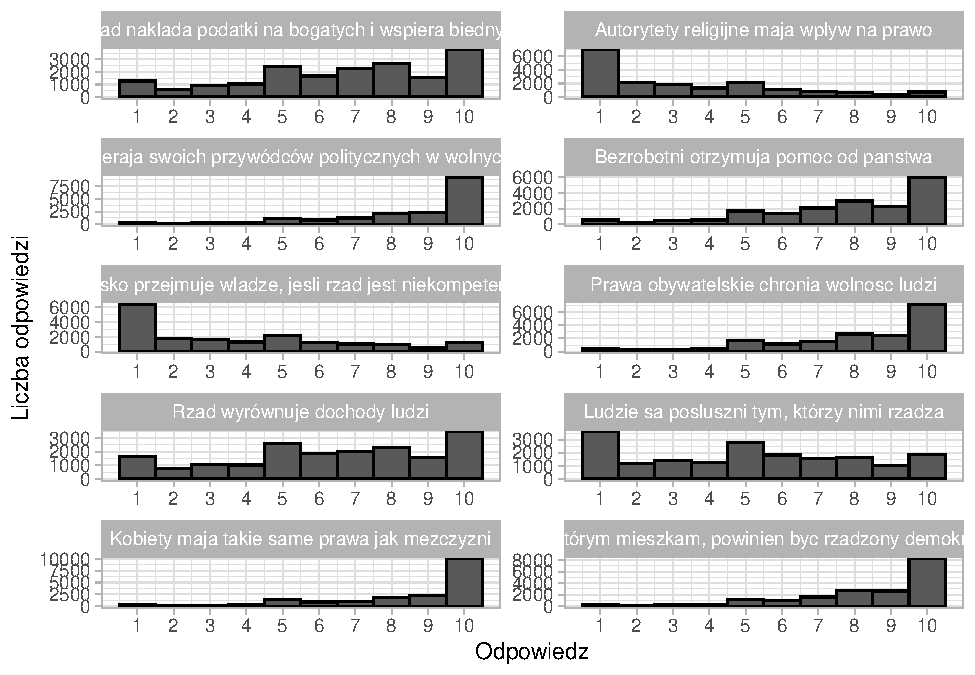
\includegraphics{text_ASA_files/figure-latex/descr-plot-1} \hfill{}

\caption{Rozkład odpowiedzi na pytania o demokrację w ankiecie WVS. Źródło: opracowanie własne.}\label{fig:descr-plot}
\end{figure}

Już ta prosta analiza opisowa pokazuje, że elitystyczna definicja demokracji Schumpetera nie jest wystarczająca w europejskich społeczeństwach. Obywatele zgodnie uważają, że demokracja nie polega tylko na wolnych wyborach, ale też służy zapewnianiu praw i wolności obywatelskich, równości płci, oraz - co najbardziej zaskakujące - pomocy bezrobotnym. Zdaniem samych wyborców, do demokracji nie wystarczy sam fakt wybrania rządzących, ale rządzący ci muszą spełniać podstawowe potrzeby wolności, równości i ekonomicznego bezpieczeństwa rządzonych.

Istnieje też powszechne mniemanie, że system demokratyczny nie potrzebuje interwencji ze strony armii ani autorytetów religijnych. Natomiast opinia społeczna jest mniej jednogłośna, jeśli chodzi o kwestię redystrybucji i rozwarstwienia dochodowego. Choć większość uważa, że w demokracji państwo powinno się tym zajmować, przewaga najwyższej odpowiedzi nie jest aż tak wyraźna.

Ciekawym przypadkiem są tu odpowiedzi na pytanie o posłuszeństwo rządzącym. Koncepcja demokracji Schumpetera pośrednio zakłada raczej posłuszeństwo wobec rządzących, którzy zostali zaakceptowani, co jest też zresztą cechą jakichkolwiek systemów rządzenia czy zarządzania.

\hypertarget{analiza-korelacji}{%
\subsection{Analiza korelacji}\label{analiza-korelacji}}

Kiedy ankietowany odpowiada na pytanie ``w jakim stopniu {[}pewna cecha{]} jest podstawową cechą demokracji?'', musi odwołać się do jakiejś koncepcji demokracji i odnieść do niej cechę, której dotyczy pytanie. Jeżeli istnieje ogólnie przyjęta społeczna koncepcja demokracji, obejmująca część spośród zawartych w pytaniach cech, można się spodziewać, że odpowiedzi na te pytania będą silnie skorelowane. Ankietowani będą odpowiadać w podobny sposób, ponieważ posiadają tę samą koncepcję demokracji. Analogicznie, jeśli nie istnieje społeczna koncepcja demokracji (to znaczy: pogląd na demokrację jest bardzo indywidualną kwestią), można się spodziewać, że siła związków między odpowiedziami na różne pytania będzie nieistotna.

Siłę tych związków mierzono współczynnikiem korelacji Spearmana. Mimo, że dane mają charakter porządkowy, można je traktować jako ciągłe ze względu na dużą liczbę punktów skali \citep{Revelle}.

Koncepcję demokracji można opisać zmienną latentną, która wpływa na odpowiedzi (zmienne mierzalne). Koncepcji może być kilka, ale nie więcej, niż pytań. Na odpowiedź na dane pytanie może wpływać więcej niż jedna koncepcja. Warto też zauważyć, że wyodrębnione z danych koncepcje są określone tylko w zakresie pytań, które zadano w ankiecie. Nie można na tej podstawie stwierdzić, czy koncepcja obejmuje też inne kwestie, np. bioetyczne. Teoretycznie mogą również istnieć koncepcje demokracji, które nie zawierają objętych pytaniami cech, wobec czego wymykają się badaniu.

Rys. 2 przedstawia macierz korelacji odpowiedzi na wszystkie pytania. Dla macierzy wykonano test sferyczności Bartletta, na podstawie którego stwierdzono, że jest istotnie różna od macierzy jednostkowej, zatem siła związków między zmiennymi jest istotna (\(\chi^2\) = 46805,62; \(df\) = 45; \(p\) \textless{} 0,001).

\begin{figure}

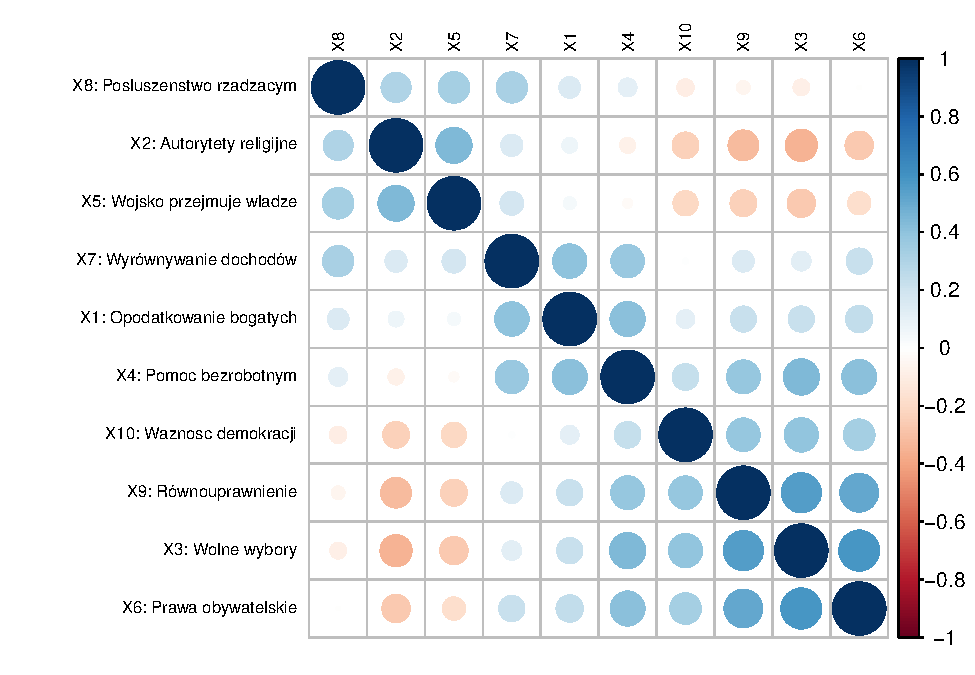
\includegraphics{text_ASA_files/figure-latex/cor-matrix-1} \hfill{}

\caption{Macierz korelacji odpowiedzi na pytania o demokrację. Źródło: opracowanie własne.}\label{fig:cor-matrix}
\end{figure}

Na Rys. 2 wyraźnie wyłaniają się trzy skupiska. Wskazują na istnienie w badanej grupie trzech odrębnych koncepcji demokracji, przejawiających się w podobnych wzorcach odpowiedzi:

\begin{itemize}
\tightlist
\item
  Koncepcja I: zmienne oznaczające posłuszeństwo rządzącym, wpływ autorytetów religijnych na prawo, możliwość przejęcia władzy przez wojsko oraz (w mniejszym stopniu) wyrównywanie dochodów;
\item
  Koncpecja II: zmienne oznaczające wyrównywanie dochodów, wyższe opodatkowanie bogatych, pomoc dla bezrobotnych;
\item
  Koncepcja III: zmienne oznaczające pomoc dla bezrobotnych, równouprawnienie płci, wolne wybory i prawa obywatelskie;
\end{itemize}

Pierwsza wizja charakteryzuje się przede wszystkim przekonaniem, że podstawową cechą demokracji jest ingerencja w działanie państwa stron trzecich, czyli autorytetów religijnych oraz wojska. Ceni również posłuszeństwo wobec rządzących. W tej koncepcji demokracji, skupionej raczej wokół porządkowania stosunków władzy, znalazło się też jednak przekonanie, że państwo powinno dbać o równy rozkład dochodów. Grupa ta jest wyraźnie negatywnie skorelowana z grupą III, a przede wszystkim - z potrzebą życia w demokratycznym państwie. Można przypuszczać, że członkowie grupy w rzeczywistości nie cenią demokracji, ale zapytani o jej istotę, i tak projektują na nią cechy swojego wymarzonego (niedemokratycznego) systemu.

Druga koncepcja przedstawia demokrację głównie jako gwaranta korzyści lub bezpieczeństwa ekonomicznego. Jej wyznawcy oczekują od państwa walki z nierównościami dochodowymi, opodatkowania najbogatszych, wsparcia dla najbiedniejszych oraz bezrobotnych. Można ten wzorzec określić jako koncepcję państwa opiekuńczego.

W ostatniej koncepcji demokracja to system, którego istotą są wolne wybory, równość i swoboda obywatelska, ale również wsparcie dla bezrobotnych. Chociaż i ta koncepcja wychodzi daleko poza definicję Schumpetera (według której jedyną podstawową cechą demokracji są wolne wybory) to jest do niej najbliższa. Wyznawcy koncepcji postrzegają demokrację jako gwarancję wolności politycznych i bardziej niż innym zależy im, żeby mieszkać w demokratycznym kraju.

Ponadto warto zauważyć, że zmienne oznaczające wyrównywanie dochodów oraz wyższe opodatkowanie bogatych charakteryzują się pozytywnymi korelacjami z niemal wszystkimi pozostałymi zmiennymi.

Warto zestawić Rys. 2 z informacjami wyniesionymi z Rys. 1. Analiza korelacji pozwala tylko wnioskować o kształcie i wewnętrznej spójności poszczególnych koncepcji, a nie o ich powszechności (ile osób jest do nich przekonanych) ani umiejscowieniu na skali odpowiedzi. Rys. 1 pozwala przypuszczać, że najbardziej powszechna jest koncepcja III i że jej wyznawcy wybierają najwyższe odpowiedzi w składających się na nią pytaniach, podczas gdy wyznawcy koncepcji I i tak wybierają generalnie niskie odpowiedzi na swoje pytania - choć nie tak niskie, jak reszta społeczeństwa. Nie można też wykluczyć, że funkcjonuje ona jako ``anty-koncepcja''; powszechnie uznawany wzorzec, jak demokracja nie powinna wyglądać.

Koncepcja II i III wydają się pokrywać z badaniami Jaśko i Kossowskiej \citeyearpar{JaskoKoss} dla polskiego społeczeństwa. Wyodrębniły one, odpowiednio: ``standard opiekuńczości'' oraz ``standard wolności''. Z kolei analizy przyczyn poparcia i zaufania ludzi do demokracji i demokratycznych rządów pokazują, że po części wynikają one z zaangażowania obywateli w działalność społeczną, częściowo ze sprzyjającej sytuacji ekonomicznej, a częściowo z psychologicznego mechanizmu, że ludzie generalnie popierają system, który już jest przyjęty, o ile nie mają silnych powodów do niezadowolenia z niego \citep{Campbell}. Poparcie dla demokracji wynikające z korzystnej sytuacji ekonomicznej jasno potwierdza, że obywatele oczekują od demokratycznego systemu, że pozwoli im żyć w ogólnie pojętym dobrobycie (koncepcja II). Po drugie, skoro ludzie ufają demokratycznym rządom dzięki możliwości zaangażowania w działalność społeczną, to można przypuszczać, że oczekują od demokracji zapewnienia swobody takiego działania. Pośrednio tę swobodę można wiązać z postulatami praw obywatelskich oraz równości płci (w kontekście emancypacji kobiet, która pozwoliła im na bardziej czynny udział w życiu społecznym), znajdującymi się w koncepcji III. Trzeci, behawioralny składnik poparcia demokracji wg. Campbella, nie jest kwestią koncepcji demokracji, więc nie ma tu zastosowania.

Można również spojrzeć na społeczne koncepcje demokracji pod kątem jej trwałości. W szczególnie burzliwych momentach dziejowych wśród badaczy popularny staje się pogląd, że świat odwraca się od demokracji, choć dane jak dotąd temu przeczą \citep{Doorenspleet}. Padają wówczas pytania, co może sprawić, że naród odrzuci formę ustroju, uważaną przecież tak powszechnie za najlepszą z możliwych. Okazuje się, że nawet gdy obywatele nie są zadowoleni ze swoich rządzących, nie są skłonni przekreślić demokratycznego systemu ich wybierania, o ile ten system zapewnia im podstawowe prawa i zaspokaja oczekiwania. Z kolei niestabilna sytuacja ekonomiczna jest poważną próbą wytrzymałości dla młodych demokracji, jak to było widoczne pod koniec XX w. w Europie Środkowo-Wschodniej \citep{Klingemann}.

To, że obywatele są gotowi odrzucić system, który nie zaspokaja oczekiwań, może brzmieć jak truizm, ale odsłania ważną niedoskonałość elitystycznej definicji Schumpetera: ludzie nie postrzegają demokracji jako systemu, który pozwala im wybrać rządzących wedle upodobania, ale jako takiego, który daje największe możliwości realizowania swoich potrzeb, zarówno społecznych jak i ekonomicznych. Wybór rządzących jest tylko środkiem do osiągnięcia celu, nie celem samym w sobie.

Pewną zagadką pozostaje kwestia koncepcji I, która wydaje się nie mieć żadnego poparcia w dotychczasowych badaniach. Na podstawie samej macierzy korelacji można by przypuszczać, że istnieje wyłącznie jako anty-koncepcja, jednak temu przeczy dalsza analiza, która pokazuje, że istnieje nieduża grupa ludzi bardziej przekonanych do tej koncepcji, niż do pozostałych.

\hypertarget{model-strukturalny}{%
\subsection{Model strukturalny}\label{model-strukturalny}}

Postać modelu przedstawiono na diagramie na Rys. 3, zgodnie ze standardem przedstawiania równań strukturalnych \citep{Everitt}. Zmienne latentne zostały oznaczone przez okręgi, zmienne mierzalne przez kwadraty, a na liniach prostych między nimi podano wartości wyestymowanych ładunków czynnikowych. Zakrzywione linie oznaczają wariancje lub kowariancje.

Ze względu na złamanie założenia o normalności zmiennych mierzalnych, model estymowano Odporną Metodą Największej Wiarygodności. Ponieważ modele ze zmiennymi latentnymi nie są ściśle identyfikowalne, o czym pisano w rozdziale 2.2, przy estymacji przyjęto jednostkową wariancję zmiennych latentnych oraz wartość pierwszego ładunku czynnikowego na 1. Na diagramie na Rys. 3 jest on wyróżniony przerywaną linią, ale wartości ładunków czynnikowych zostały zestandaryzowane dla wygodniejszej interpretacji. Wszystkie współczynniki są istotne.

\begin{figure}

{\centering 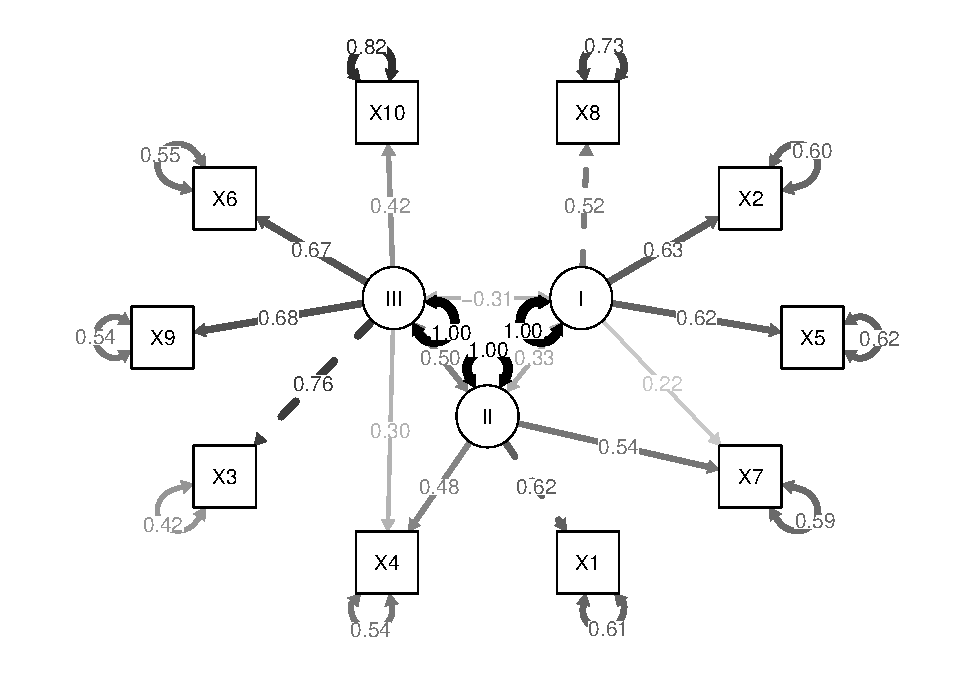
\includegraphics{text_ASA_files/figure-latex/diagram-all-1} 

}

\caption{Diagram modelu analizy czynnikowej koncepcji demokracji. Źródło: opracowanie własne.}\label{fig:diagram-all}
\end{figure}

I koncepcja najsilniej przejawia się w zmiennych oznaczających wpływ autorytetów religijnych na prawo oraz możliwość przejęcia władzy przez wojsko. II jest wyrażana przede wszystkim w poparciu opodatkowania bogatych i wsparcia ubogich. Koncepcja III wyraża się głównie przez docenienie wagi wolnych wyborów, a na drugim miejscu: równość płci i prawa obywatelskie. Koncepcje II i III są ze sobą pozytywnie skorelowane na średnim poziomie (0,5). Koncepcja I jest słabo, ale dodatnio skorelowana z II, oraz równie słabo, ale ujemnie, z koncepcją III.

Model posiada dość dobre własności. CFI = 0,953, jest więc na dobrym poziomie, ale TLI wynosi tylko 0,930. RMSEA wynosi 0,057; CI90\% (0,055; 0,060), co również jest bardzo korzystną wartością. Łączna rzetelność konstruktu (Composite Reliability) wynosi 0,74, co oznacza, że pytania są dobrze dobrane do badanych koncepcji.

Dla każdej obserwacji w zbiorze można teraz obliczyć liczbową wartość każdej koncepcji jako średnią ważoną, gdzie wagami są standaryzowane ładunki czynnikowe. Taki wskaźnik można interpretować jako miarę tego, jak bardzo ankietowany zgadza się z daną koncepcją. Rys. 4 przedstawia, jak kształtują się te wskaźniki w całej grupie.

\begin{figure}

{\centering 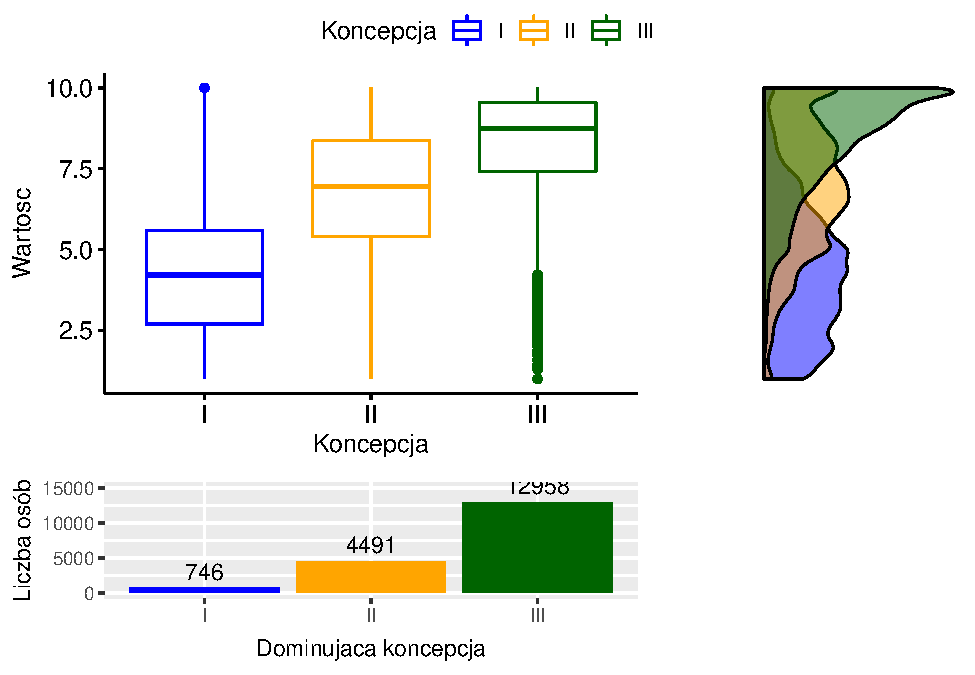
\includegraphics{text_ASA_files/figure-latex/stats-all-1} 

}

\caption{Rozkład wartości wskaźników koncepcji demokracji (na górze) i liczby osób, u których dana koncepcja była dominująca (na dole). Źródło: opracowanie własne.}\label{fig:stats-all}
\end{figure}

Wyraźnie widać, że ludzie najmniej zgadzają się z koncepcją I (średnia 4,28) następnie II (średnia 6,85), a najbardziej z III (średnia 8,3). Przypadki, kiedy wskaźnik tej ostatniej jest poniżej 4 to wartości odstające, więc można powiedzieć, że prawie nie ma ludzi, którzy by się z tą koncepcją nie zgadzali. Policzono również obserwacje, w których najwyższą wartość mają wskaźniki poszczególnych koncepcji (wykres na dole). Zdecydowanie najwięcej jest ludzi, dla których najważniejsza jest koncepcja III.

Pytanie brzmi, czy model jest równoważny pomiarowo, a więc czy można zastosować te wskaźniki do mierzenia różnic w postrzeganiu demokracji między krajami. W celu przetestowania pierwszego poziomu równoważności - równoważność konfiguralna - podjęto próbę estymacji tego samego modelu dla każdego kraju osobno. Okazało się, że w niektórych grupach (dla Gruzji i Słowenii) model nie mógł się poprawnie wyestymować, co oznacza, że postać modelu nie pasuje do danych. To oznacza, że równoważność konfiguralna nie jest zachowana.

W celu uzyskania wspólnego, międzynarodowego konceptu demokracji można by wykluczyć z badania kraje, dla których model okazał się nieidentyfikowalny, i ponowić procedurę. Takie rozwiązanie jest jednak tylko pominięciem problemu. Nie ma wspólnej dla europejskich społeczeństw koncepcji demokracji (obejmującej kwestie wymienione w rozdziale 4.2). Przyjęcie koncepcji powstałych przez nakładanie się na siebie koncepcji różnych państw i odrzucenie najbardziej odstających krajów nie daje zbyt wiele informacji o naturze różnic.

Można jednak przypuszczać, że istnieją w Europie grupy państw o wystarczająco zbliżonych poglądach na demokrację, że można w nich używać wspólnych konstruktów. W następnych rozdziałach podjęto próbę znalezienia takich grup, modelowania występujących w nich koncepcji i pokazania różnic.

\newpage

\hypertarget{podziaux142-paux144stw-wedux142ug-przebiegu-ux17celaznej-kurtyny}{%
\section{Podział państw według przebiegu Żelaznej Kurtyny}\label{podziaux142-paux144stw-wedux142ug-przebiegu-ux17celaznej-kurtyny}}

\hypertarget{linia-podziaux142u}{%
\subsection{Linia podziału}\label{linia-podziaux142u}}

W poprzednim rozdziale zbudowano model koncepcji demokracji dla grupy wszystkich ujętych w badaniu państw, ale wykazano też, że koncepcje nie występują w identycznej formie we wszystkich państwach. W tym rozdziale zostanie podjęta próba wyodrębnienia mniejszych grup, w których przypuszczalnie mogą występować wspólne koncepcje.

Można przypuszczać, że różnice wynikają z historycznych uwarunkowań. Spora część państw europejskich w drugiej połowie XX wieku znajdowała się w komunistycznej strefie wpływów (tzw. demokracje ludowe), podczas gdy inne pozostały kapitalistyczne i rozwijała się w nich idea tzw. demokracji liberalnej. Dlatego podjęto próbę podziału na następujące grupy:
- demokracje liberalne: Niemcy, Holandia i Szwecja (oznaczone na Rys. 5 kolorem żółtym);
- byłe demokracje ludowe: Polska, Estonia, Białoruś, Ukraina, Słowenia, Rumunia, Gruzja, Kazachstan i Rosja (oznaczone na Rys. 5 kolorem fioletowym);
- Turcja i Hiszpania to przypadki, które nie pasują do żadnej z grup;

\begin{figure}
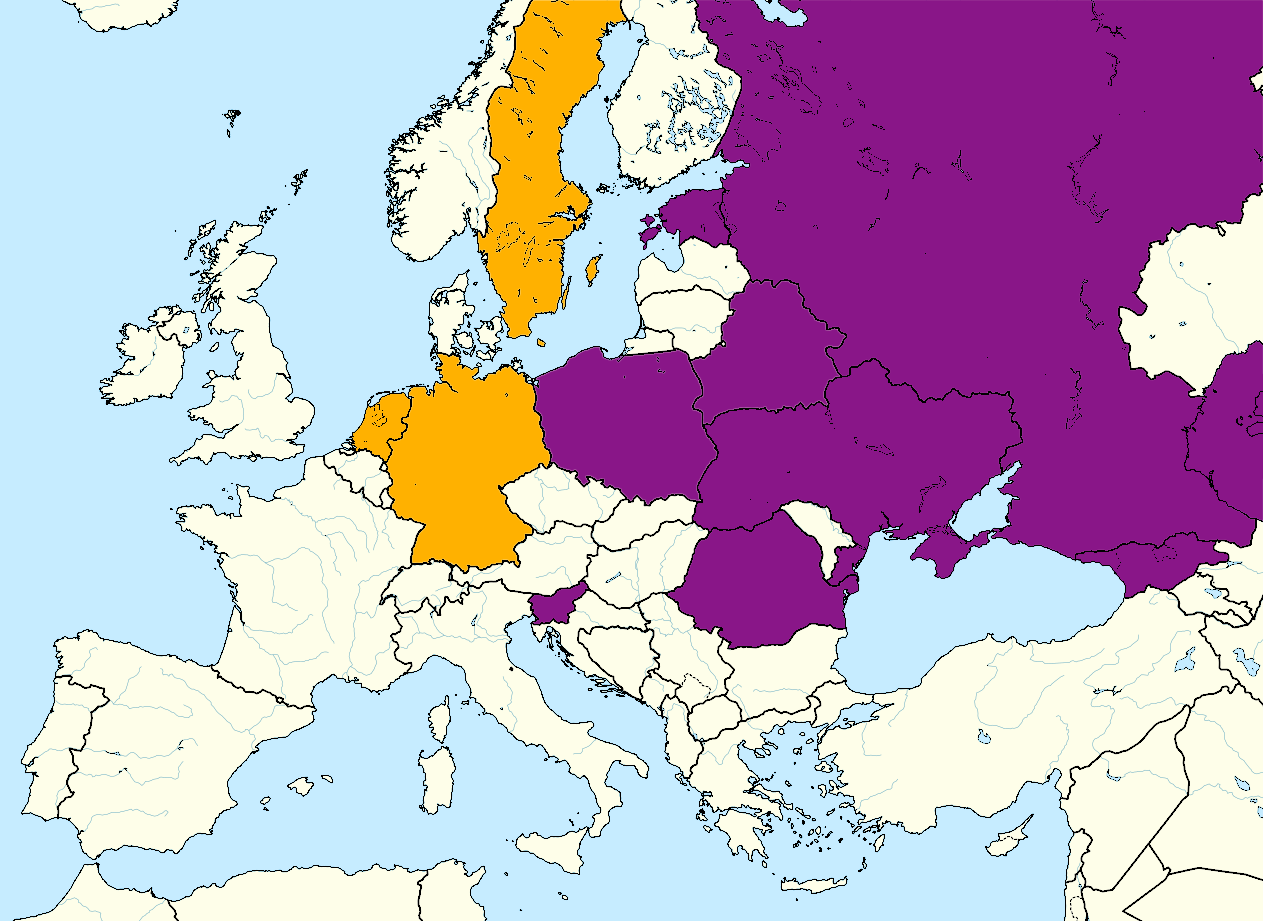
\includegraphics[width=450px]{map1} \caption{Mapa podziału na grupy według przebiegu Żelaznej Kurtyny. Źródło: opracowanie własne.}\label{fig:map1}
\end{figure}

\hypertarget{koncepcje-demokracji-w-grupie-demokracji-liberalnych}{%
\subsection{Koncepcje demokracji w grupie demokracji liberalnych}\label{koncepcje-demokracji-w-grupie-demokracji-liberalnych}}

Grupa demokracji liberalnych zawiera tylko trzy państwa: Niemcy, Holandię i Szwecję; jest też bardzo skupiona pod względem geograficznym. Test sferyczny Bartletta pokazał, że macierz korelacji jest istotnie różna od macierzy jednostkowej (\(\chi^2\) = 10186,17; \(df\) = 45; \(p\) \textless{} 0,001). Na Rys. 6 można zauważyć podobne wzorce, jak w grupie ogólnej. Powiązania ze zmiennymi mierzalnymi przedstawiono na diagramie na Rys. 7.

\begin{figure}

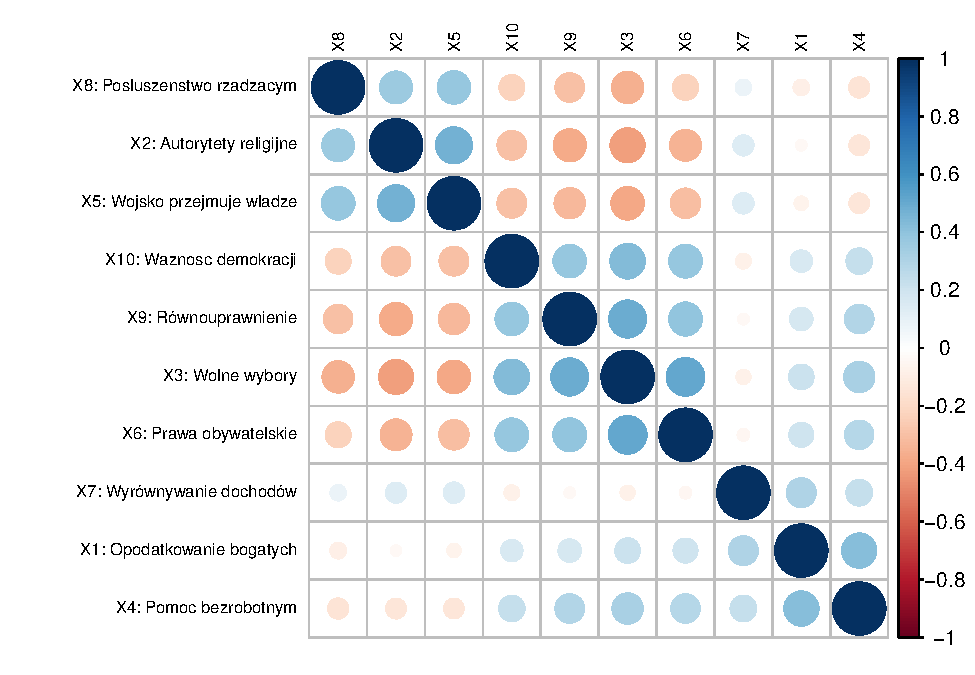
\includegraphics{text_ASA_files/figure-latex/cor-matrix-lib-1} \hfill{}

\caption{Macierz korelacji odpowiedzi na pytania o demokrację w grupie demokracji liberalnych. Źródło: opracowanie własne.}\label{fig:cor-matrix-lib}
\end{figure}

W tej grupie występują koncepcje II i III, opisane wcześniej. Ostatnia koncepcja ma nieco inną strukturę (przedstawioną na diagramie Rys. 7), dlatego zostanie oznaczona jako Ilib. Dopasowanie modelu do danych jest bardzo dobre. CFI (Robust Comparative Fit Index) = 0,965; TLI (Robust Tucker-Lewis Index) = 0,950. RMSEA wynosi 0,043; CI90\% (0,038; 0,049). Łączna rzetelność konstruktu wynosi 0,62, jest więc dość niska. Model w tej grupie charakteryzuje się silną ujemną korelacją między koncepcją III a Ilib, oraz brakiem związku między koncepcją II a pozostałymi.

\begin{figure}

{\centering 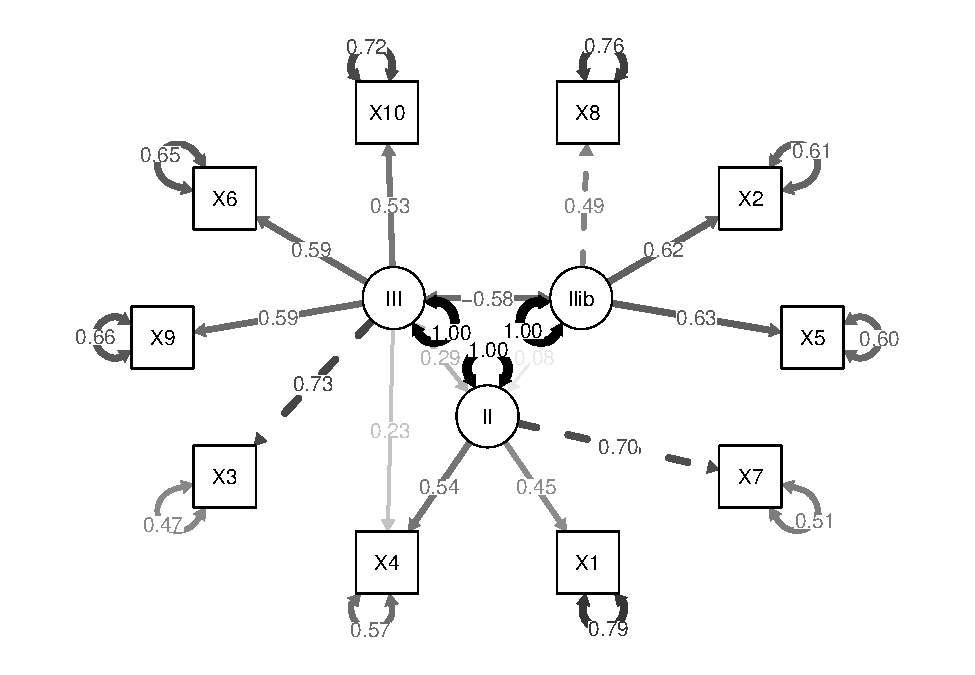
\includegraphics{text_ASA_files/figure-latex/diagram-west-1} 

}

\caption{Diagram modelu analizy czynnikowej koncepcji demokracji w grupie demokracji liberalnych. Źródło: opracowanie własne.}\label{fig:diagram-west}
\end{figure}

Rozkłady wskaźników w tej grupie przedstawiono na Rys. 8. Koncepcja Ilib ma średnią na poziomie 2,56, a wartości powyżej 7 są bardzo rzadkie. Koncepcja II ma średnią 6,11. III ma 8,7, a wartości poniżej 6 są przypadkami odstającymi.

\begin{figure}

{\centering 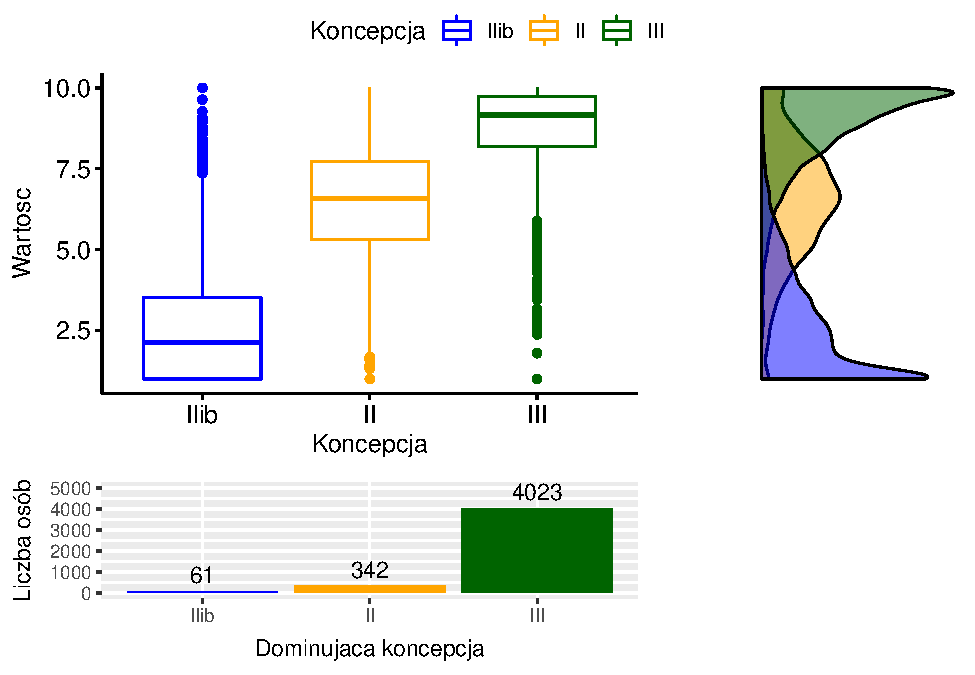
\includegraphics{text_ASA_files/figure-latex/stats-west-1} 

}

\caption{Rozkład wartości wskaźników koncepcji demokracji (na górze) i liczby osób, u których dana koncepcja była dominująca (na dole) w grupie demokracji liberalnych. Źródło: opracowanie własne.}\label{fig:stats-west}
\end{figure}

Tabela 2 przedstawia wyniki równoważności pomiarowej. Zachowana jest wyłącznie równoważność konfiguralna, co potwierdza istnienie tych samych koncepcji demokracji we wszystkich społeczeństwach państw grupy.

\begin{table}

\caption{\label{tab:tab-west}Wyniki analizy równoważności pomiarowej dla grupy demokracji liberalnych. Źródło: opracowanie własne.}
\centering
\resizebox{\linewidth}{!}{
\begin{tabular}[t]{l|r|r|l|l|r|l}
\hline
Poziom równoważności & AIC & BIC & \$\textbackslash{}chi\textasciicircum{}2\$ & Przyrost \$\textbackslash{}chi\textasciicircum{}2\$ & Stopnie swobody & p-value\\
\hline
Konfiguralna & 180493 & 181145 & 458,66 &  & 93 & \\
\hline
Metryczna & 180611 & 181161 & 608,95 & 150,29 & 109 & < 2,2e-16\\
\hline
Skalarna & 181894 & 182354 & 1919,63 & 1310,68 & 123 & < 2.2e-16\\
\hline
\end{tabular}}
\end{table}

Analiza równoważności pomiarowej pokazuje, że choć każda zmienna wynika z tej samej koncepcji we wszystkich krajach, to siła tego związku jest w różnych krajach różna. Oznacza to, że w państwach należących do grupy demokracji liberalnych występują te same społeczne koncepcje demokracji, jednak model nie pozwala na rzetelne porównywanie ich poziomów między państwami, ani bezpośrednio, ani w relacji z innymi zmiennymi.

\hypertarget{koncepcje-demokracji-w-grupie-byux142ych-demokracji-ludowych}{%
\subsection{Koncepcje demokracji w grupie byłych demokracji ludowych}\label{koncepcje-demokracji-w-grupie-byux142ych-demokracji-ludowych}}

Grupa państw, które znajdowały się w komunistycznej strefie wpływów, jest znacznie liczniejsza. Jej macierz korelacji przedstawia wykres Rys. 9 . Test sferyczny Bartletta potwierdził, że jest istotnie różna od macierzy jednostkowej (\(\chi^2\) = 27891,81; \(df\) = 45; \(p\) \textless{} 0,001). Można wyodrębnić trzy koncepcje. Koncepcja III, taka jak w grupie ogólnej; koncepcja II z dodatkiem zmiennej oznaczającej posłuszeństwo rządzącym, tu oznaczona jako IIlud; oraz koncepcja Ilib. Bazując na macierzy korelacji, z początku połączono zmienne oznaczające wyrównywanie dochodów i opodatkowanie bogatych ze zmiennymi koncepcji III, ale w wyestymowanym modelu okazały się one nieistotne. (opodatkowanie bogatych: \(Z\) = -0,011; \(p\) = 0,992; wyrównywanie dochodów: \(Z\) = -1,225; \(p\) = 0,221).

\begin{figure}

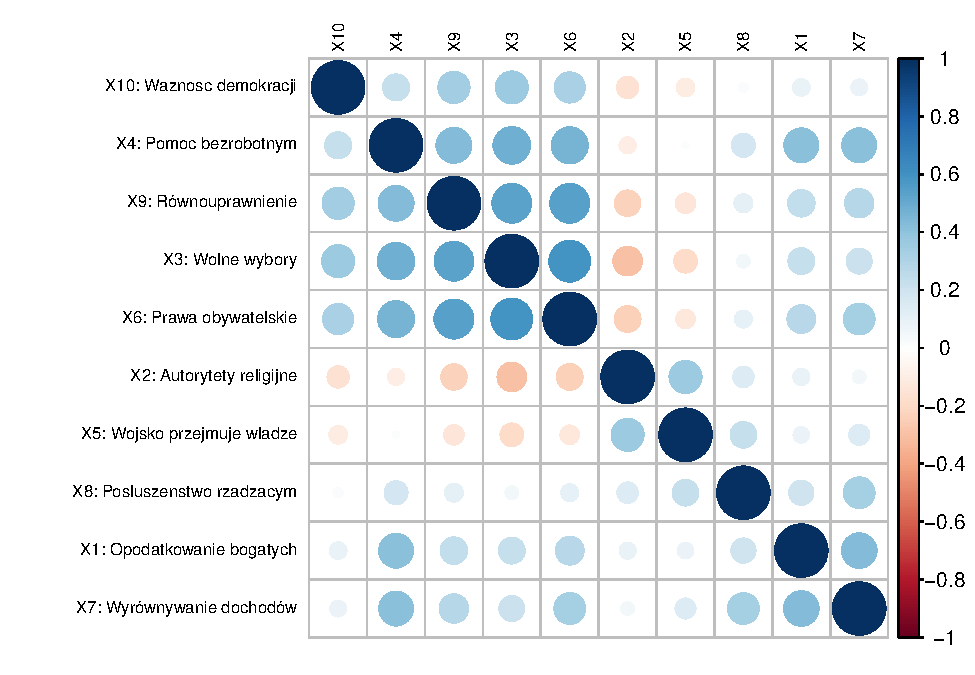
\includegraphics{text_ASA_files/figure-latex/cor-matrix-east-1} \hfill{}

\caption{Macierz korelacji odpowiedzi na pytania o demokrację w grupie byłych demokracji ludowych. Źródło: opracowanie własne.}\label{fig:cor-matrix-east}
\end{figure}

Ostateczną postać modelu przedstawia diagram na Rys. 10. CFI (Robust Comparative Fit Index) = 0,966; TLI (Robust Tucker-Lewis Index) = 0,948. RMSEA wynosi 0,049; CI90\% (0,045; 0,052). Łączna rzetelność konstruktu wynosi 0,76. Model dla tej grupy jest bardzo dobrze dopasowany do danych.

\begin{figure}

{\centering 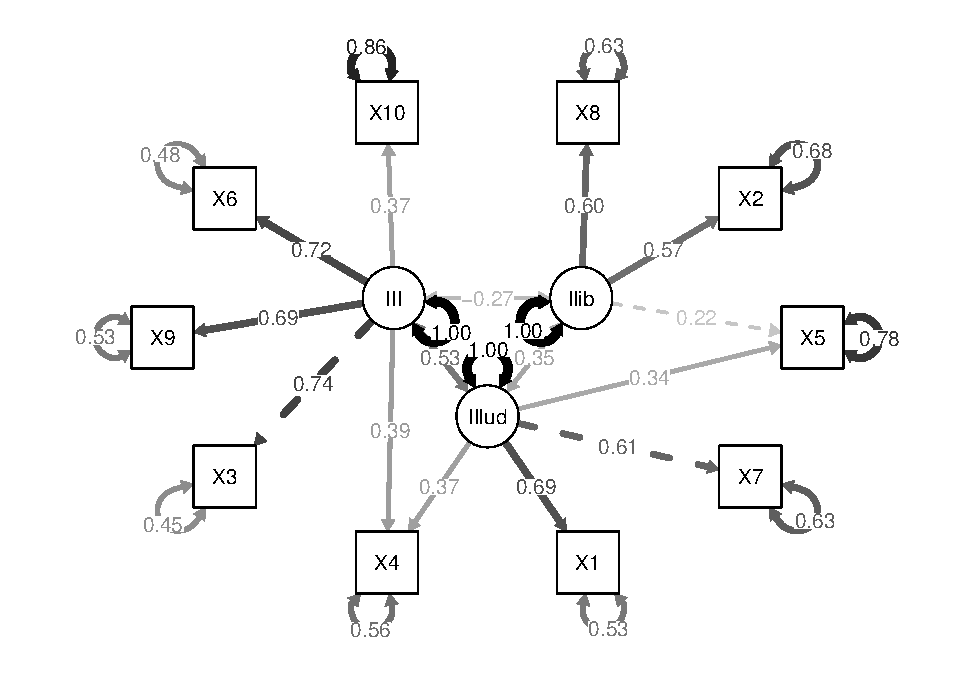
\includegraphics{text_ASA_files/figure-latex/diagram-east-1} 

}

\caption{Diagram modelu analizy czynnikowej koncepcji demokracji w grupie byłych demokracji ludowych. Źródło: opracowanie własne.}\label{fig:diagram-east}
\end{figure}

Jednak nie udało się poprawnie wyestymować modelu w każdym kraju z osobna. Równoważność konfiguralna nie jest zachowana, co oznacza, że zilustrowana diagramem na Rys. 10 struktura koncepcji demokracji nie występuje w każdej z byłych demokracji ludowych.

\newpage

\hypertarget{podziaux142-wedux142ug-podobieux144stwa-macierzy-korelacji}{%
\section{Podział według podobieństwa macierzy korelacji}\label{podziaux142-wedux142ug-podobieux144stwa-macierzy-korelacji}}

\hypertarget{metoda-podziaux142u}{%
\subsection{Metoda podziału}\label{metoda-podziaux142u}}

W poprzednim rozdziale pokazano, że linia podziału wyznaczona przez Żelazną Kurtynę nie dała grup o wspólnych koncepcjach demokracji. Jej drugą istotną wadą było odrzucenie dwóch państw, których losy w drugiej połowie XX wieku wyłamywały się z tego schematu.

Zaproponowano więc zgrupowanie państw według podobieństwa występujących w nich związków między zmiennymi. Dla każdego obliczono macierz korelacji i wykonano grupowanie hierarchiczną metodą aglomeracyjną AGNES. Wyniki przedstawia dendrogram na Rys. 11. Na początku algorytmu każde państwo jest traktowane jako odrębne skupisko (dolna część dendrogramu). W każdym kolejnym kroku obliczana jest euklidesowa odległość między średnimi wartościami zmiennych dla każdej pary skupisk, a następnie dwa najbliżesze skupiska zostają połączone w jedno. Algorytm kończy się, gdy wszystkie państwa zostaną zebrane w jednym skupisku (szczyt dendrogramu) \citep{Struyf}.

Wysokość jest tu miarą odległości dwóch skupisk, które zostają ze sobą połączone \citep{MaechRouss}. Kraje, które łączą się ze sobą na najniższej wysokości, mają najbardziej podobne wzorce odpowiedzi - zatem można podejrzewać, że na odpowiedzi mają wpływ te same ukryte koncepcje demokracji.

\begin{figure}

{\centering 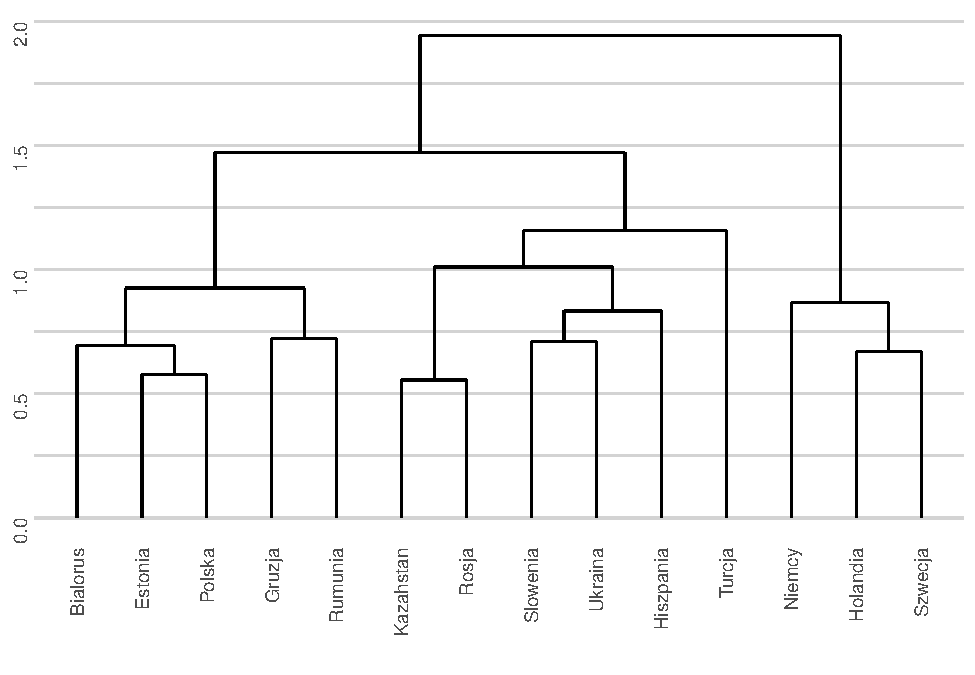
\includegraphics{text_ASA_files/figure-latex/dendrogram-1} 

}

\caption{Grupowanie państw według podobieństwa macierzy korelacji metodą aglomeracyjną. Źródło: opracowanie własne.}\label{fig:dendrogram}
\end{figure}

Na Rys. 11 widać trzy wyraźnie wyodrębnione grupy. Pierwszą (oznaczoną na mapie kolorem zielonym) tworzą państwa Europy środkowo-wschodniej oraz Gruzja; drugą (oznaczoną na czerwono) głównie państwa leżące nad Morzem Czarnym, ale też Słowenia i Hiszpania. Trzecia grupa (oznaczoną na niebiesko) składa się z krajów północno-zachodniej Europy i pokrywa się z grupą demokracji liberalnych, która została już przeanalizowana w poprzednim rozdziale. Wzorzec geograficzny jest więc wyraźny, ale nie pozbawiony wyjątków, co widać na Rys. 12. Dużą przeszkodą w wyciąganiu ogólnych wniosków jest ograniczony zasięg badania. Z większości państw zachodniej oraz południowej Europy nie ma danych, i trudno przewidzieć, jakie wzorce występują w tych rejonach.

\begin{figure}
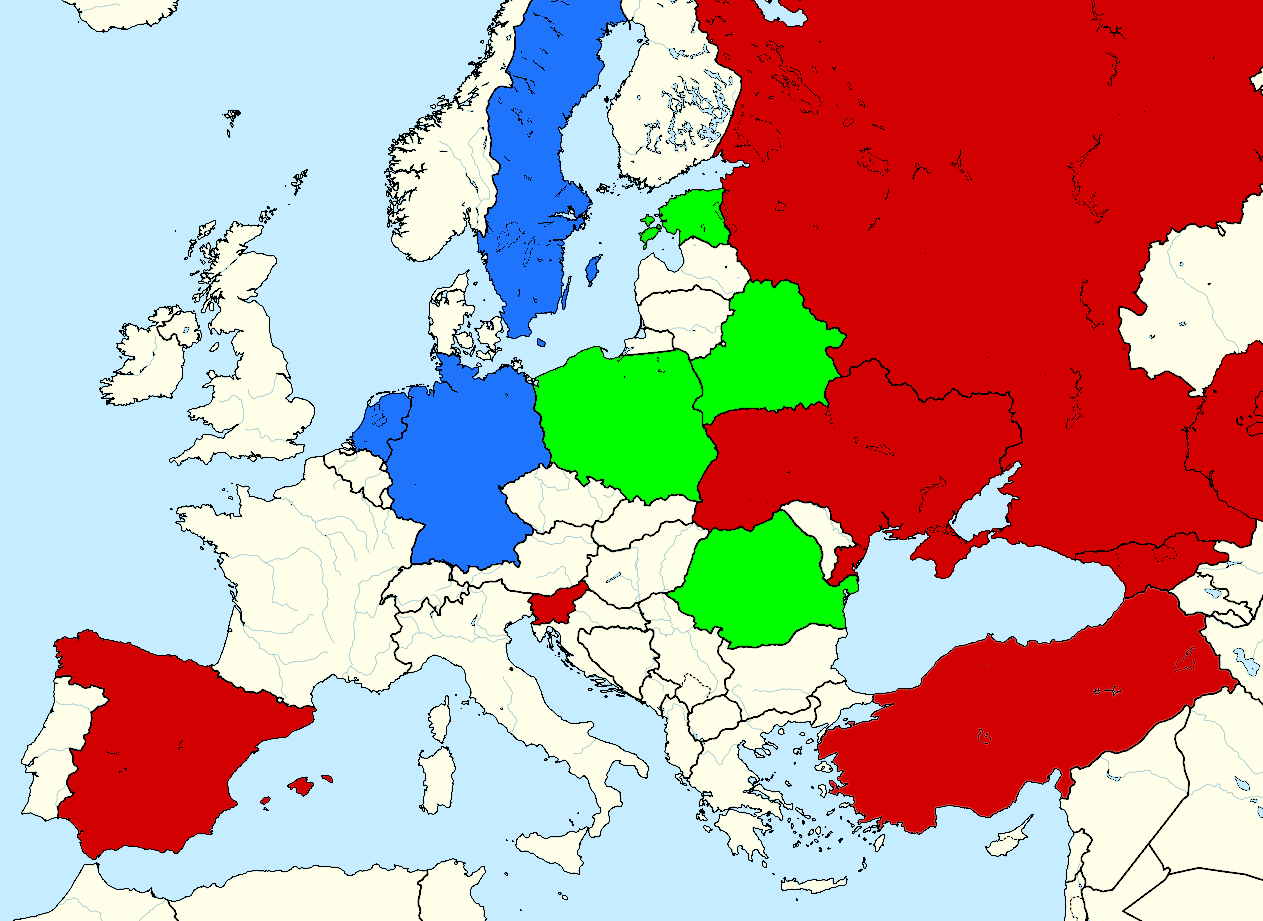
\includegraphics[width=450px]{map2} \caption{Mapa podziału na grupy według podobieństwa macierzy korelacji. Źródło: opracowanie własne.}\label{fig:map2}
\end{figure}

Jakość grupowania sprawdzono, obliczając wskaźnik sylwetkowy dla każdego kraju (Rys. 13). Wskaźnik przyjmuje wartości od -1 do 1, gdzie ujemne stanowią przesłankę, że obserwacja została umieszczona w niewłaściwej grupie, dodatnie - we właściwej, a zerowe oznaczają obserwacje, które nie pasują do żadnej z grup \citep{Rousseeuw}. Jak można zauważyć na wykresie, nie ma podstaw do przeniesienia któregokolwiek kraju do innej grupy. Z drugiej strony, wartości generalnie są niskie, co oznacza, że rozgrupowanie nie jest bardzo wyraźne. Najbliższe zeru wartości mają Turcja (0,017), Słowenia (0,039) i Hiszpania (0,102) w czerwonej grupie. Żeby nie tracić dużej ilości danych, zdecydowano się jednak pozostawić grupy w ich pierwotnym składzie, jeśli nie spowoduje to później problemów z estymacją.

\begin{figure}

{\centering 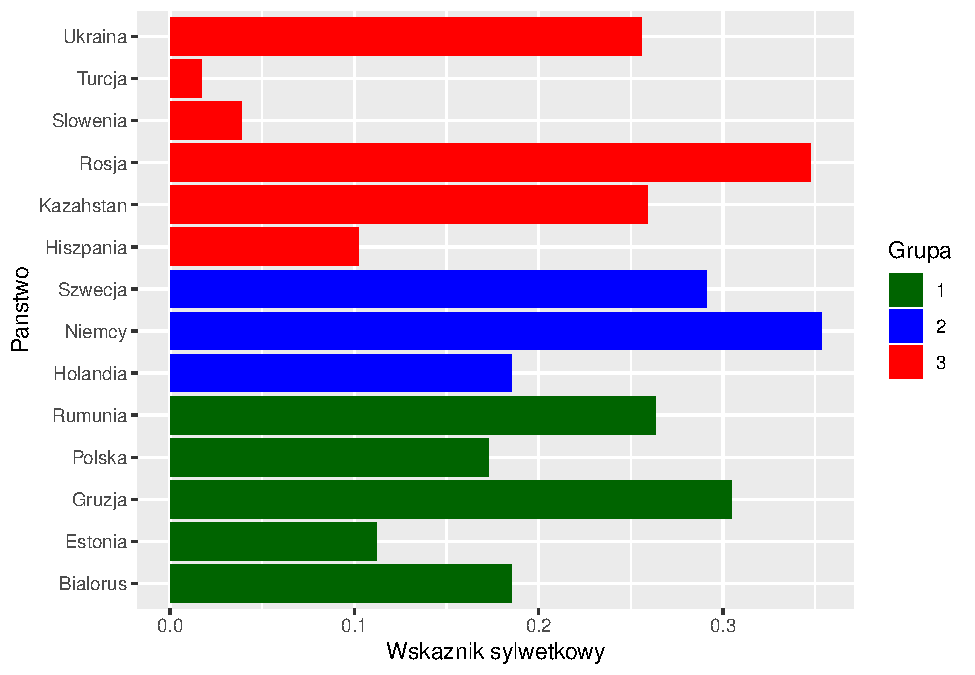
\includegraphics{text_ASA_files/figure-latex/silhouette-1} 

}

\caption{Test sylwetkowy grupowania, Źródło: opracowanie własne.}\label{fig:silhouette}
\end{figure}

\hypertarget{grupa-oznaczona-na-zielono}{%
\subsection{Grupa oznaczona na zielono}\label{grupa-oznaczona-na-zielono}}

Pierwsza grupa składa się z pięciu państw: Polski, Białorusi, Estonii, Rumunii i Gruzji. Kraje te łączą liczne podobieństwa, przede wszystkim komunistyczne rządy i wpływy Związku Radzieckiego po II Wojnie Światowej oraz rewolucyjne zmiany w latach 80. i 90. XX wieku.

Test sferyczny Bartletta pokazał, że macierz korelacji jest istotnie różna od macierzy jednostkowej (\(\chi^2\) = 12861,33; \(df\) = 45; \(p\) \textless{} 0,001). Relacje między odpowiedziami są dość podobne do wzorca dla wszystkich krajów. Nadal można wyodrębnić trzy koncepcje, chociaż nieco mniej wyraźne.

\begin{figure}

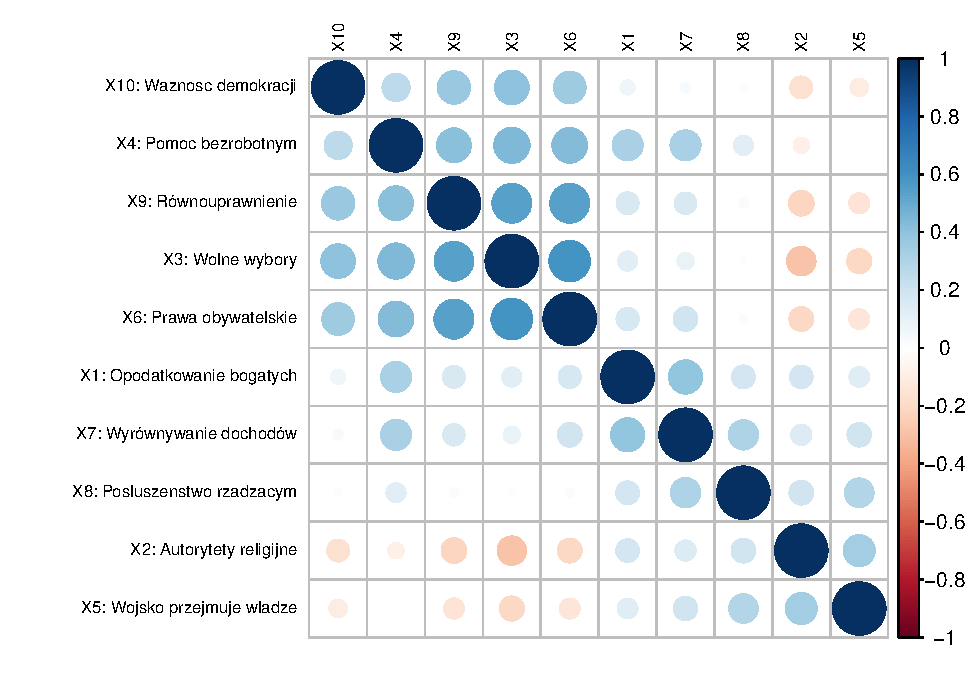
\includegraphics{text_ASA_files/figure-latex/cor-matrix-1-1} \hfill{}

\caption{Macierz korelacji odpowiedzi na pytania o demokrację w grupie oznaczonej na zielono. Źródło: opracowanie własne.}\label{fig:cor-matrix-1}
\end{figure}

Postać modelu i wyniki estymacji przedstawiono na diagramie na Rys. 14. CFI (Robust Comparative Fit Index) = 0,969; TLI (Robust Tucker-Lewis Index) = 0,953. RMSEA wynosi 0,045; CI90\% (0,040; 0,050). Łączna rzetelność konstruktu wynosi 0,75. Dopasowanie modelu w tej grupie jest więc lepsze niż dla całej próby.

W tej grupie występuje koncepcja IIlud ze zmienną posłuszeństwo rządzącym, ale wyraźnie większe znaczenie ma w niej wyrównywanie przez państwo dochodów. Można interpretować to jako wizję paternalistycznego państwa, które wymaga posłuszeństwa, ale zaspokaja podstawowe potrzeby bytowe i chroni najsłabszych przed wyzyskiem. Warto też zwrócić uwagę na układ korelacji między zmiennymi latentnymi: w grupie ogólnej i grupie demokracji liberalnych koncepcje opiekuńczego państwa były silniej związane z koncepcją III - tutaj z koncepcją I.

\begin{figure}

{\centering 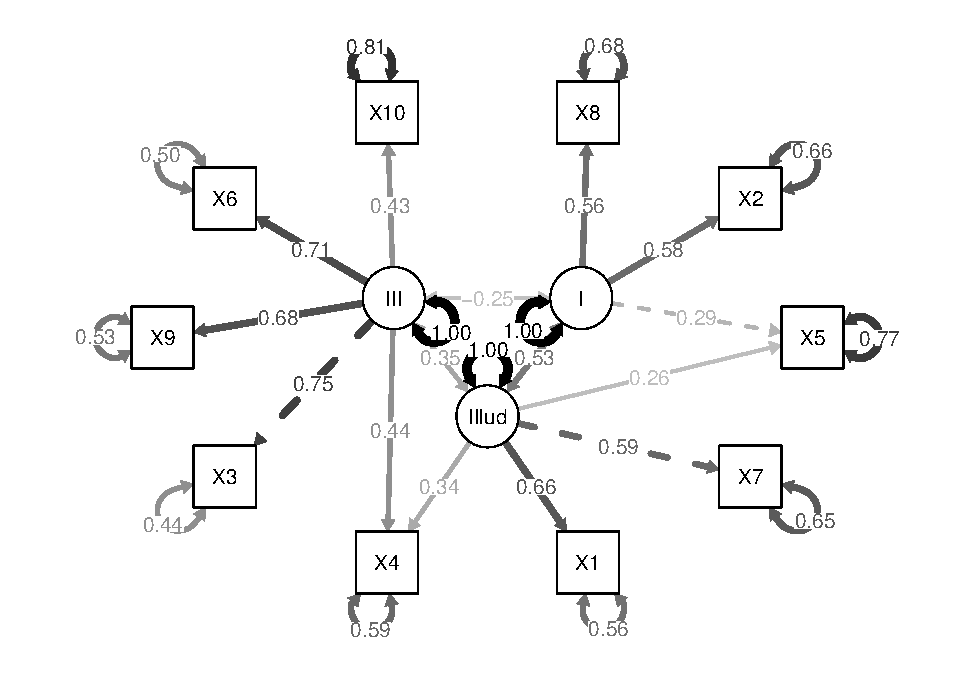
\includegraphics{text_ASA_files/figure-latex/diagram-1-1} 

}

\caption{Diagram modelu analizy czynnikowej koncepcji demokracji w grupie oznaczonej na zielono. Źródło: opracowanie własne.}\label{fig:diagram-1}
\end{figure}

Średnia wartość wskaźnika koncepcji I to 4,16, IIlud - 6,14, III - 8,08.

\begin{figure}

{\centering 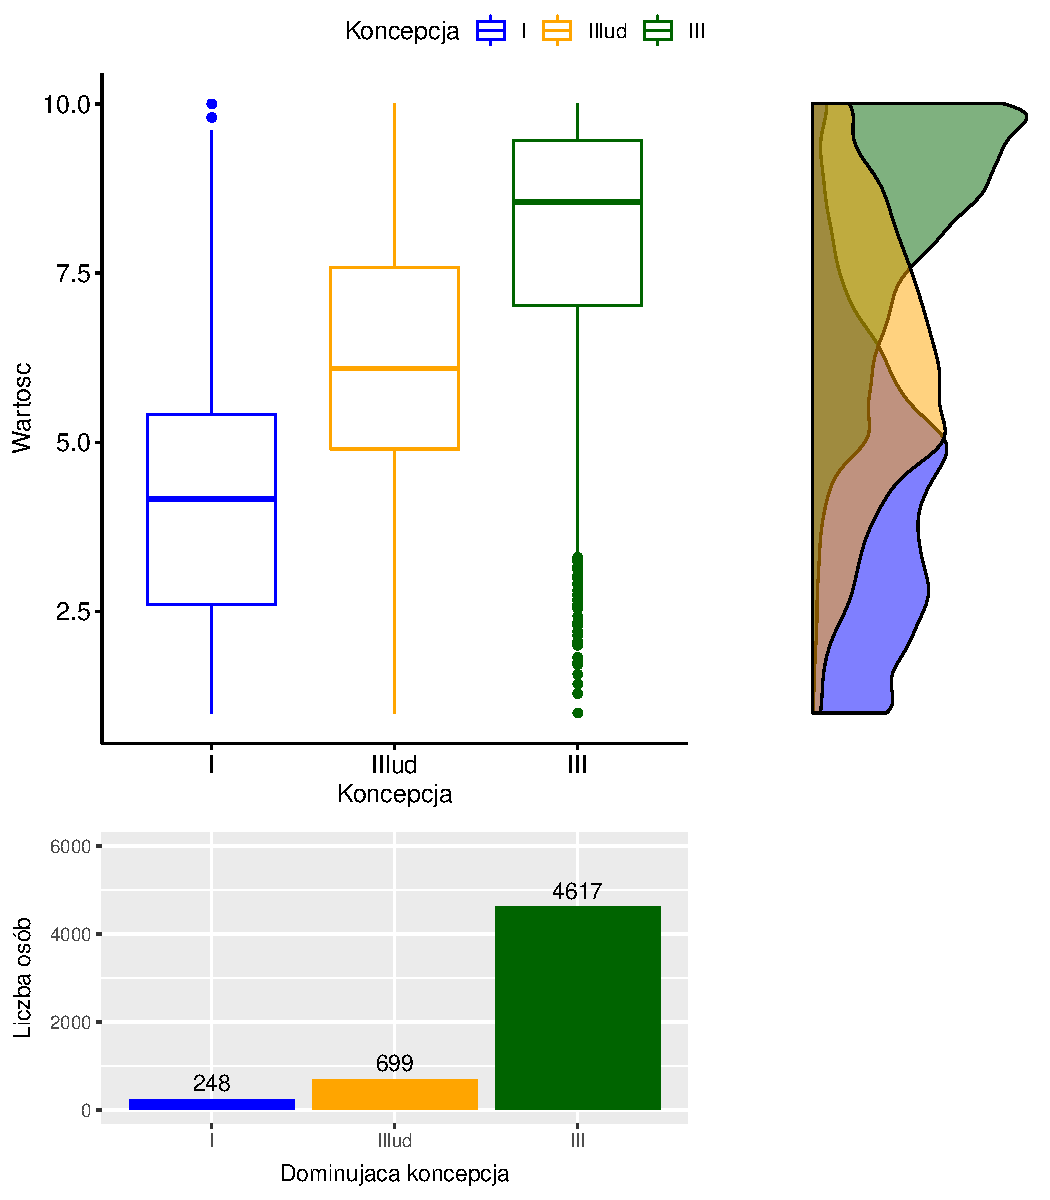
\includegraphics{text_ASA_files/figure-latex/stats-gr-1-1} 

}

\caption{Rozkład wartości wskaźników koncepcji demokracji (na górze) i liczby osób, u których dana koncepcja była dominująca (na dole) w grupie oznaczonej na zielono. Źródło: opracowanie własne.}\label{fig:stats-gr-1}
\end{figure}

Wyniki analizy równoważności pomiarowej przedstawia tabela Tabela 3.

\begin{table}

\caption{\label{tab:tab-gr-1}Wyniki analizy równoważności pomiarowej dla grupy oznaczonej na zielono. Źródło: opracowanie własne.}
\centering
\resizebox{\linewidth}{!}{
\begin{tabular}[t]{l|r|r|l|l|r|l}
\hline
Poziom równoważności & AIC & BIC & \$\textbackslash{}chi\textasciicircum{}2\$ & Przyrost \$\textbackslash{}chi\textasciicircum{}2\$ & Stopnie swobody & p-value\\
\hline
Konfiguralna & 249265 & 250325 & 1714,8 &  & 165 & \\
\hline
Metryczna & 249434 & 250255 & 1955,7 & 240,81 & 201 & < 2,2e-16\\
\hline
Skalarna & 250656 & 251266 & 3242,4 & 1286,74 & 233 & < 2.2e-16\\
\hline
\end{tabular}}
\end{table}

W każdym z państw tej grupy model przedstawiony na Rys. 14 jest identyfikowalny. Jednak modele z restrykcjami nałożonymi na, kolejno: ładunki czynnikowe i wyrazy wolne, okazały się istotnie gorsze (\(p\) \textless{} 0,001 w obu przypadkach). Równoważność metryczna i skalarna nie są spełnione.

Analiza równoważności pomiarowej pokazuje, że w państwach należących do grupy zielonej występują te same społeczne koncepcje demokracji, jednak model nie pozwala na rzetelne porównywanie ich poziomów między państwami, ani bezpośrednio, ani w relacji z innymi zmiennymi.

\hypertarget{grupa-oznaczona-na-czerwono}{%
\subsection{Grupa oznaczona na czerwono}\label{grupa-oznaczona-na-czerwono}}

Drugą grupę tworzą cztery kraje Europy Wschodniej: Ukraina, Rosja, Kazachstan i Turcja, oraz Słowenia i Hiszpania. Dla grupy obliczono macierz korelacji, przedstawioną na Rys. 15. Test Bartletta pokazał, że jest istotnie różna od macierzy jednostkowej (\(\chi^2\) = 22256,39; \(df\) = 45; \(p\) \textless{} 0,001).

Tym razem z analizy korelacji wyłaniają się tylko dwa czynniki: koncepcja I oraz zupełnie nowa koncepcja IV, której struktura została pokazana na diagramie na Rys. 16. Charakterystyczne dla tej grupy są pozytywne korelacje zmiennej oznaczającej posłuszeństwo rządzącym ze wszystkimi pozostałymi zmiennymi - przeciwnie niż w grupie demokracji liberalnych.

\begin{figure}

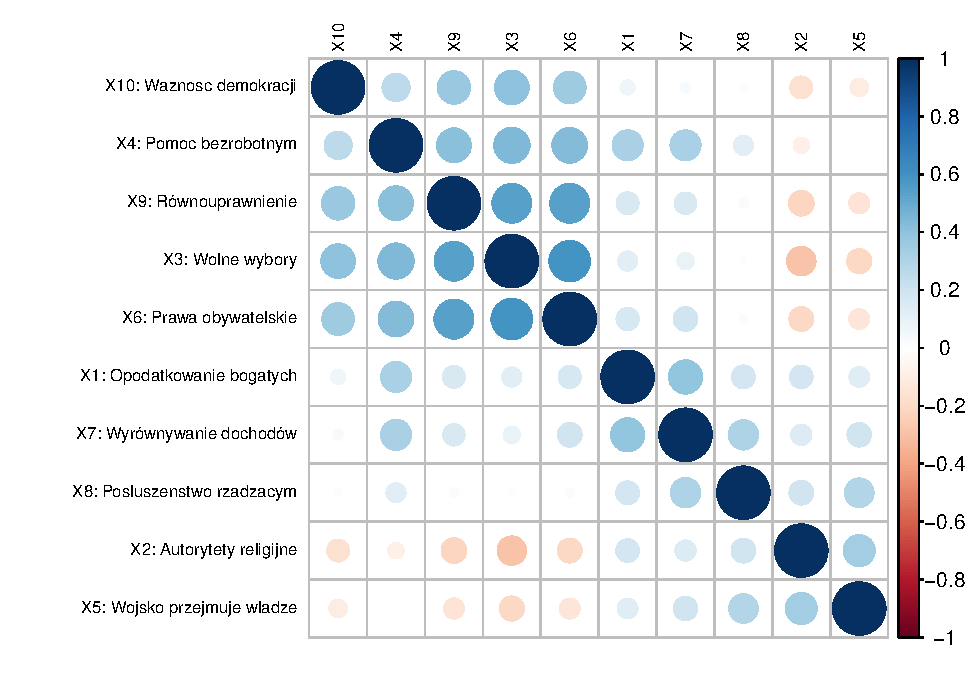
\includegraphics{text_ASA_files/figure-latex/cor-matrix-3-1} \hfill{}

\caption{Macierz korelacji odpowiedzi na pytania o demokrację w grupie oznaczonej na czerwono. Źródło: opracowanie własne.}\label{fig:cor-matrix-3}
\end{figure}

CFI (Robust Comparative Fit Index) = 0,876; TLI (Robust Tucker-Lewis Index) = 0,831. RMSEA wynosi 0,091; CI90\% (0,087; 0,099). Łączna rzetelność konstruktu wynosi 0,74. Modelu w tej grupie nie można uznać za dobrze dopasowany do danych. O ile koncepcja IV jest dobrze skonstruowana (rzetelność konceptu na poziomie 0,78), o tyle najwyraźniej brakuje odpowiednich pytań dla koncepcji I (rzetelność 0,56).

W koncepcji I najważniejsza jest interpretacja prawa przez autorytety religijne, a w IV wolne wybory, równość płci i prawa obywatelskie (część liberalna gra większą rolę niż ekonomiczna). Zmienna oznaczająca posłuszeństwo rządzącym w podobny sposób mierzy obie koncepcje. Prawdopodobnie to właśnie ta grupa ``psuła'' europejską jednorodność w definiowaniu demokracji.

\begin{figure}

{\centering 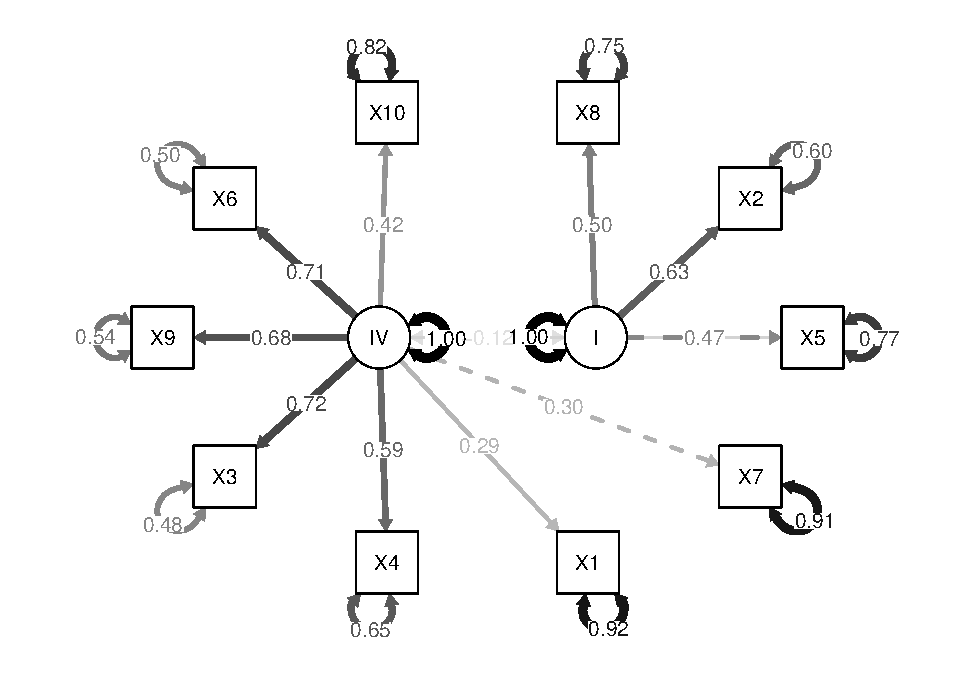
\includegraphics{text_ASA_files/figure-latex/diagram-3-1} 

}

\caption{Diagram modelu analizy czynnikowej koncepcji demokracji w grupie oznaczonej na czerwono. Źródło: opracowanie własne.}\label{fig:diagram-3}
\end{figure}

Rozkład wskaźników dla całej grupy, przedstawiony na Rys. 17, pokazuje, że koncepcja IV jest bardziej powszechna. Średnia dla koncepcji I wynosi 4,56 a dla IV - 7,77.

\begin{figure}

{\centering 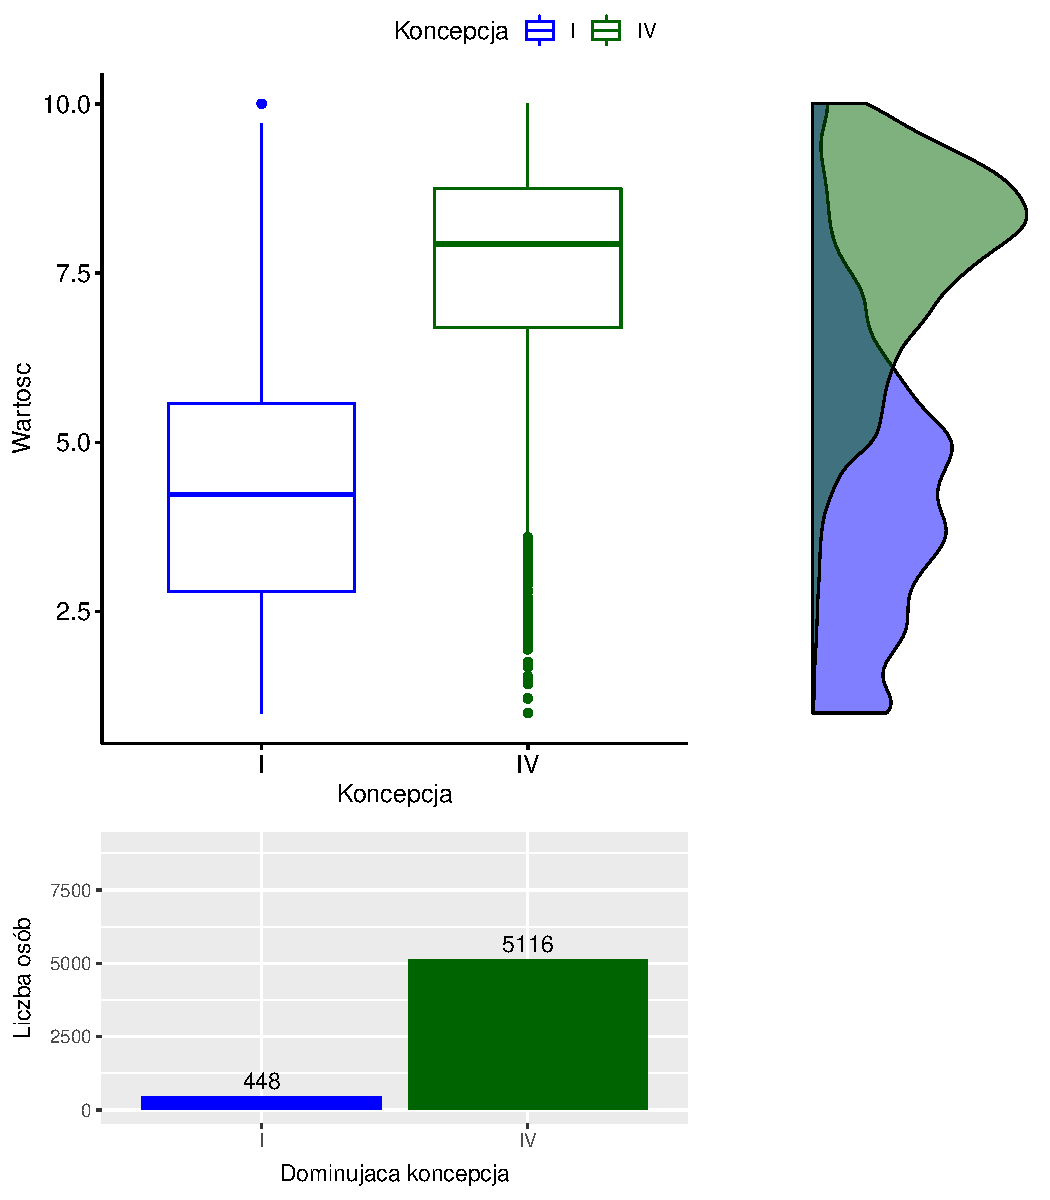
\includegraphics{text_ASA_files/figure-latex/stats-gr-3-1} 

}

\caption{Rozkład wartości wskaźników koncepcji demokracji (na górze) i liczby osób, u których dana koncepcja była dominująca (na dole) w grupie oznaczonej na czerwono. Źródło: opracowanie własne.}\label{fig:stats-gr-3}
\end{figure}

Wyniki analizy równoważności pomiarowej przedstawia tabela Tabela 4.

\begin{table}

\caption{\label{tab:tab-gr-3}Wyniki analizy równoważności pomiarowej dla grupy oznaczonej na czerwono. Źródło: opracowanie własne.}
\centering
\resizebox{\linewidth}{!}{
\begin{tabular}[t]{l|r|r|l|l|r|l}
\hline
Poziom równoważności & AIC & BIC & \$\textbackslash{}chi\textasciicircum{}2\$ & Przyrost \$\textbackslash{}chi\textasciicircum{}2\$ & Stopnie swobody & p-value\\
\hline
Konfiguralna & 361023 & 362370 & 2498,0 &  & 198 & \\
\hline
Metryczna & 361393 & 362423 & 2957,1 & 459,1 & 243 & < 2,2e-16\\
\hline
Skalarna & 363453 & 364203 & 5097,1 & 2140,0 & 283 & < 2.2e-16\\
\hline
\end{tabular}}
\end{table}

W każdym z państw tej grupy model przedstawiony na Rys. 16 jest identyfikowalny. Jednak modele z restrykcjami nałożonymi na, kolejno: ładunki czynnikowe i wyrazy wolne, okazały się istotnie gorsze (\(p\) \textless{} 0,001 w obu przypadkach). Równoważność metryczna i skalarna nie są spełnione.

\newpage

\hypertarget{podsumowanie}{%
\section{Podsumowanie}\label{podsumowanie}}

Przeprowadzona analiza czynnikowa dostarcza szeregu wniosków o społecznych koncepcjach demokracji w krajach europejskich. Przede wszystkim pokazuje, że we wszystkich krajach społeczne przekonanie o tym, co stanowi istotę demokracji, wychodzi daleko poza minimalistyczną definicję Schumpetera.

Zestaw koncepcji demokracji, którymi kierują się obywatele, nie jest wspólny dla badanych państw Europy. Znaleziono jednak trzy grupy, wewnątrz których występują wspólne koncepcje. W każdej z tych grup dalsze poziomy równoważności nie są spełnione, nie pozwalając na przeprowadzanie analiz porównawczych między krajami.

W grupie państw, w których po II Wojnie Światowej rozwijała się idea demokracji liberalnej (Niemcy, Holandia, Szwecja) można wyróżnić trzy koncepcje demokracji. Według koncepcji I istotna dla demokracji jest możliwość przejęcia władzy przez wojsko, interpretacja prawa przez autorytety religijne oraz posłuszeństwo rządzącym. Według II najistotniejsze jest, aby państwo wyżej opodatkowało bogatych i pomagało ubogim, a także wspierało bezrobotnych i walczyło z rozwarstwieniem dochodowym. W koncepcji III istotę demokracji stanowią wolne wybory, równość płci, prawa obywatelskie oraz (w mniejszym stopniu) również wsparcie państwa dla bezrobotnych. Ta trzecia koncepcja jest zdecydowanie najbardziej powszechna i silnie ujemnie skorelowana z pierwszą.

Druga grupa składa się z Polski, Estonii, Rumunii, Białorusi i Gruzji. Wyróżniono w niej również trzy koncepcje, I i III wymienione wyżej, oraz koncepcję IIlud, podobną do II. W koncepcji IIlud na pierwsze miejsce wybija się tu walka z nierównościami dochodowymi. W niedużym, ale istotnym stopniu, jest w niej też zawarte przekonanie o konieczności posłuszeństwa wobec rządzących. Koncepcja IIlud jest silnie pozytywnie skorelowana z I, nie ma z kolei związków tych dwóch koncepcji z III. Można przypuszczać, że na kształt tych koncepcji miała wpływ komunistyczna przeszłość państw tej grupy, sprawiając, że postulaty socjalne są związane z posłuszeństwem wobec władzy i możliwością przejęcia władzy przez armię. Zdecydowanie więcej jest jednak zwolenników koncepcji III.

Trzecia grupa jest najbardziej zróżnicowana pod względem geograficznym, politycznym i historycznym. Znajdują się w niej państwa: Hiszpania, Słowenia, Ukraina, Turcja, Kazachstan i Rosja. W tej grupie znaleziono tylko dwie koncepcje demokracji: jedna łączy oczekiwania wolności, równości i praw obywatelskich z postulatami socjalnymi (koncepcja IV); druga uznaje za istotne przede wszystkim wpływ autorytetów religijnych na prawo, możliwość przejęcia władzy przez armię i (w mniejszym stopniu) posłuszeństwo rządzącym (koncepcja I). Te dwie koncepcje są niezależne od siebie i IV jest bardziej powszechna. Ciekawa jest też istotność i podobny poziom ładunków czynnikowych zmiennej oznaczającej posłuszeństwo rządzącym w obu koncepcjach. W tej grupie przekonanie o konieczności posłuszeństwa wobec rządzących jest powszechne.

Dodatkowo można zauważyć, że niezależnie od grupy, wtrącanie się stron trzecich (przejęcie władzy przez wojsko oraz wpływ autorytetów religijnych na prawo) są częścią tej samej koncepcji. Z kolei wsparcie państwa dla bezrobotnych wszędzie występuje zarówno w koncepcjach skupionych na prawach politycznych i równości, jak i postulatach socjalnych.

Przeszkodą w wyciąganiu ogólnych wniosków jest brak danych dla pozostałych państw europejskich; szczególnie niedoreprezentowana jest Europa Zachodnia. Nie można również zakładać, że wszystkie istniejące społeczne koncepcje demokracji zamykają się w tych dziesięciu pytaniach, które znalazły się w ankiecie. Przeprowadzone badanie, mimo ograniczeń, rzuca jednak trochę światła na podobieństwa i różnice w tym, co jest powszechnie uważane za trzon systemu demokratycznego.

\newpage

\bibliographystyle{agsm}
\bibliography{bibliography}

\end{document}
